\onehalfspacing
\chapter{A Cronotus felhasználói felülete}

\section{A fogadó oldal és a regisztráció}

A webalkalmazásra való látogatás során a felhasználókat egy egyszerű felület fogadja, ahol lehetőségük van új felhasználó regisztrálására,
vagy belépésre egy már meglévő felhasználóval. Ez látható a \ref{fig:landing_page}-es ábrán.

\begin{figure}[h]
	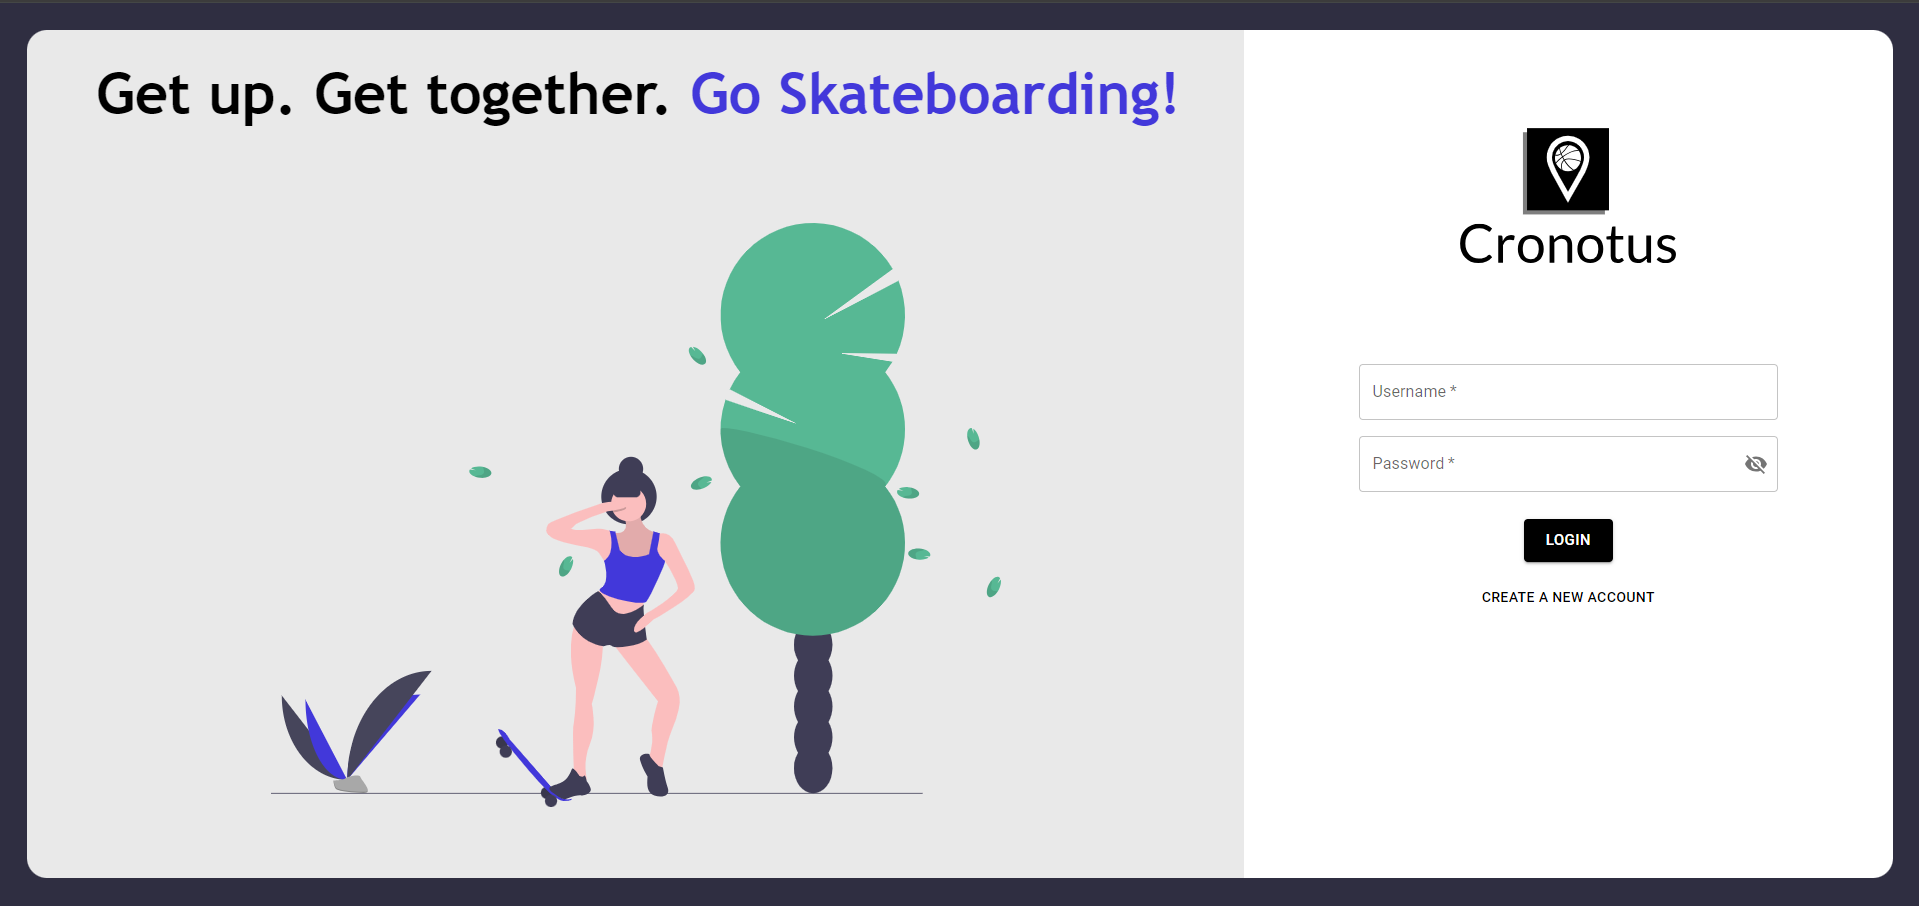
\includegraphics[width=0.5\textwidth]{images/login_page.png}
	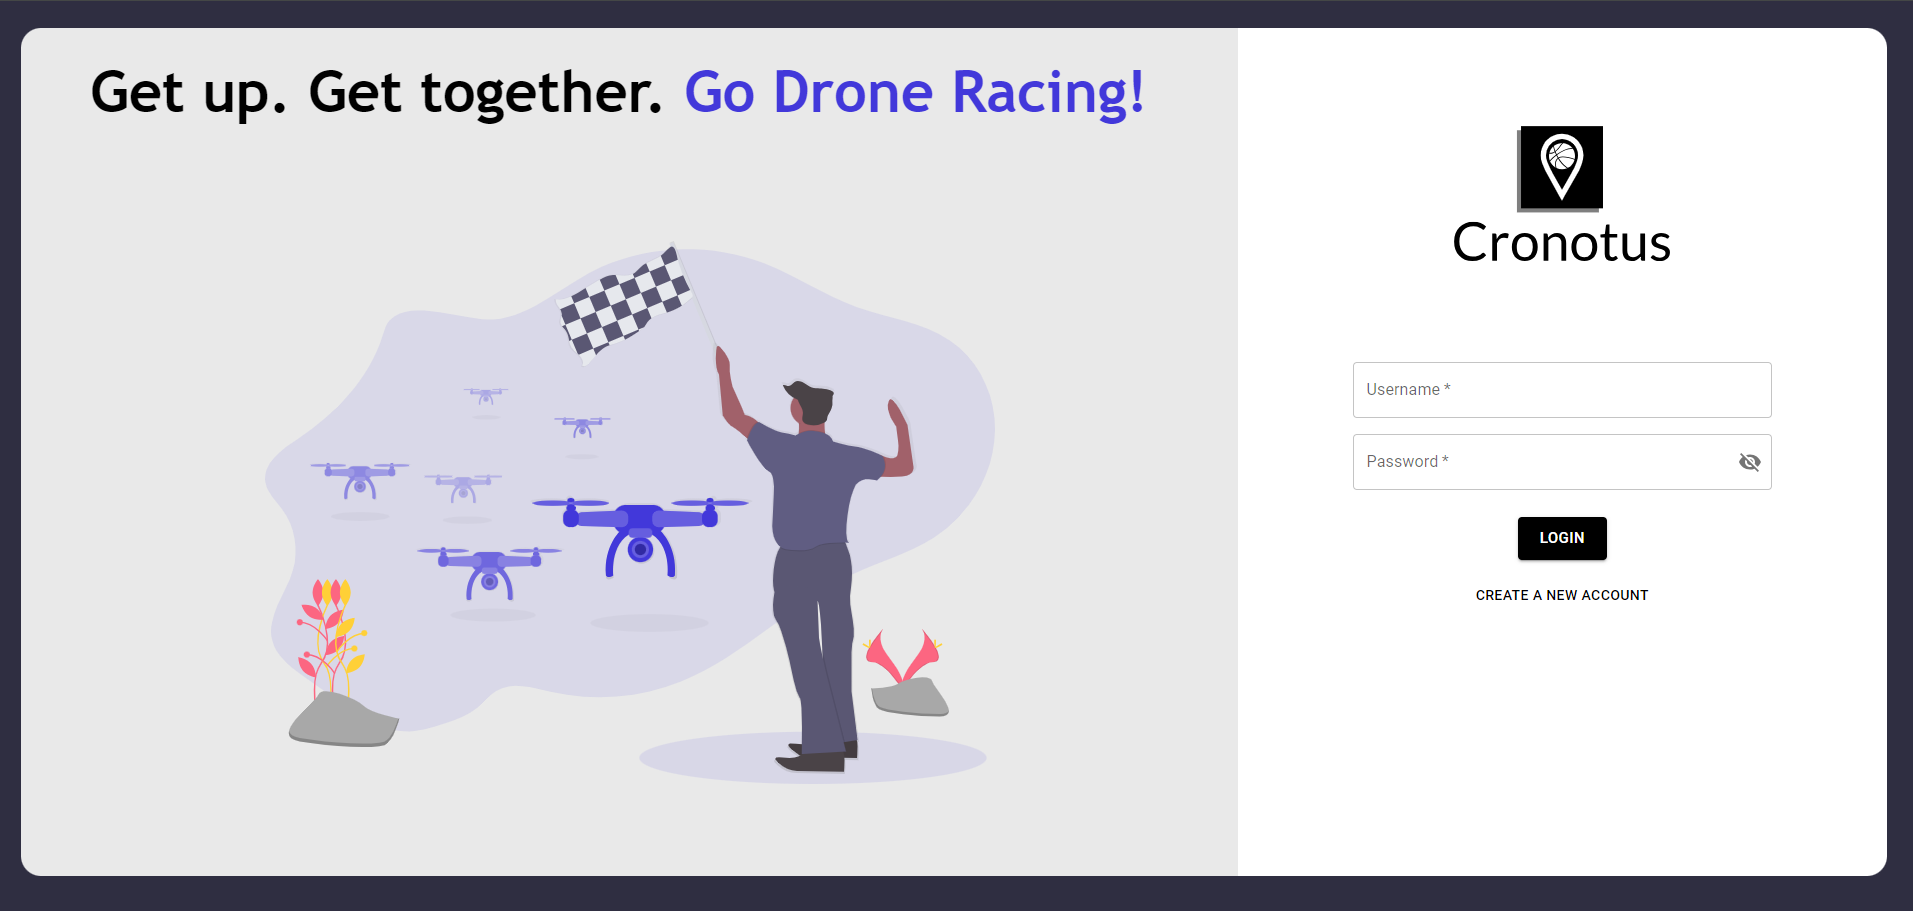
\includegraphics[width=0.5\textwidth]{images/login_2.png}
	\begin{center}
		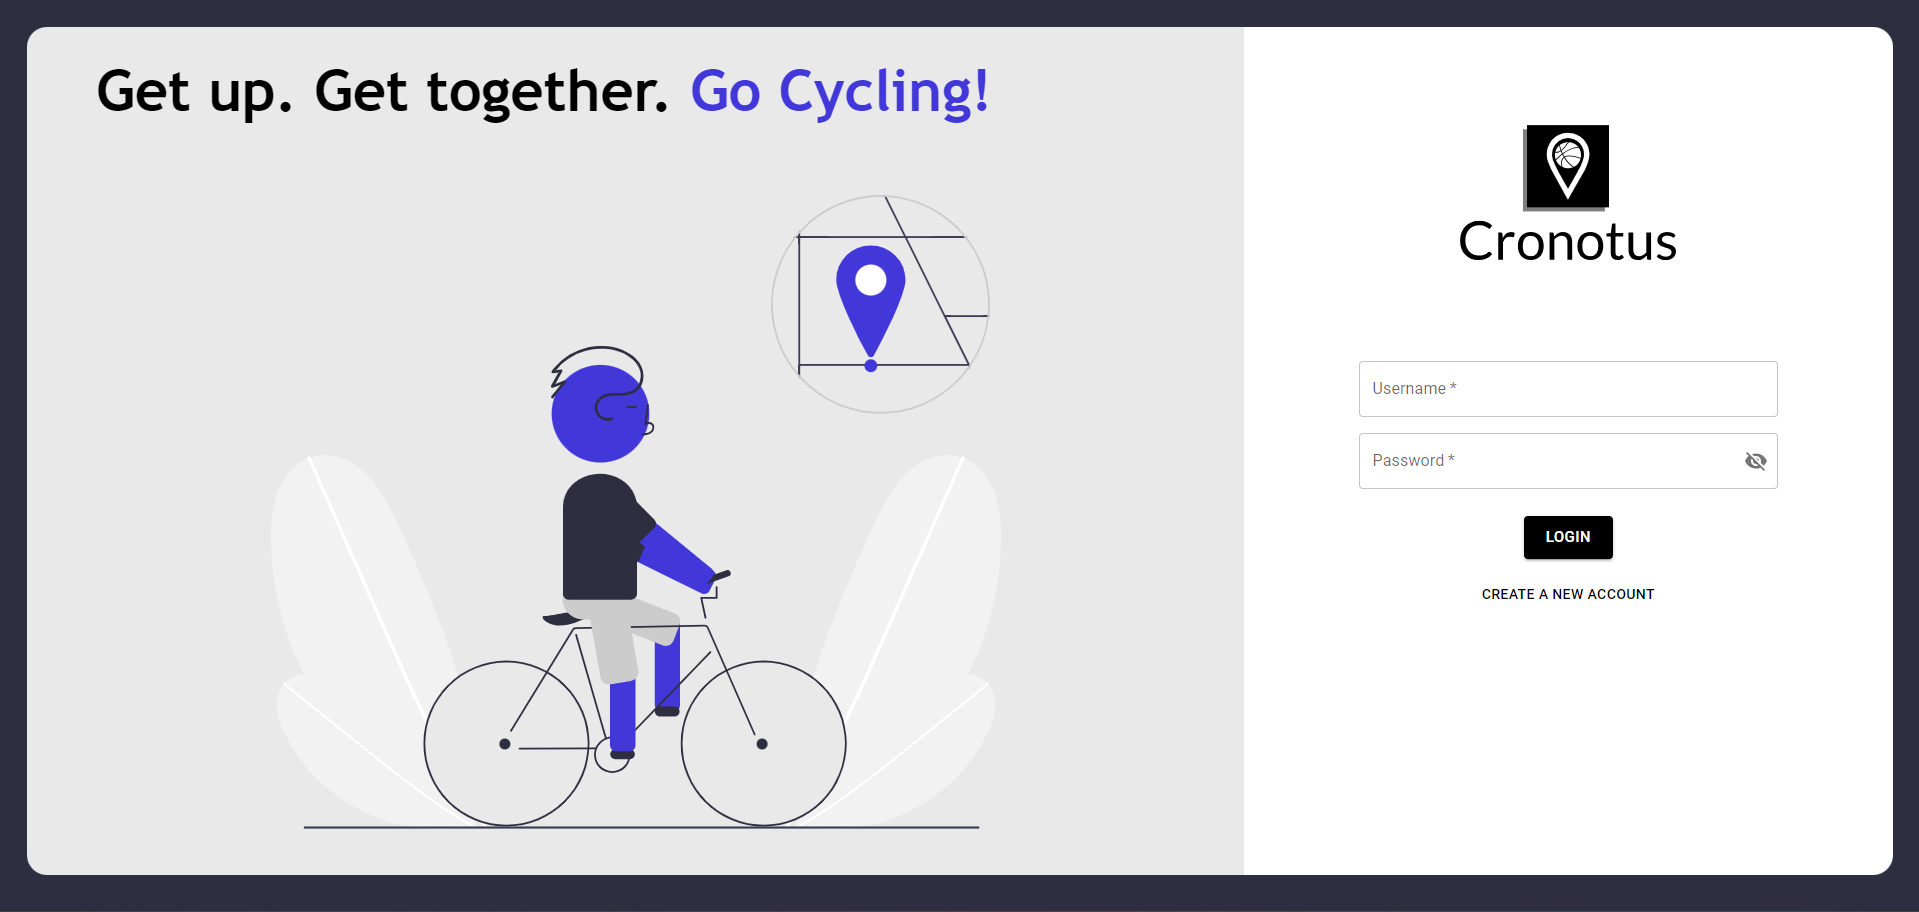
\includegraphics[width=0.7\textwidth]{images/login_3.png}
	\end{center}
	\caption{A fogadó oldal}
	\label{fig:landing_page}
\end{figure}

\newpage


A webalkalmazás igyekszik egy játékos és barátságos hangnemben megnyilvánulni a felhasználók számára. Ez megfigyelhető a regisztrációs folyamaton
is, ami nem egy megszokott űrlap kitöltéséből áll, hanem egyszerű nyelvezettel megfogalmazott kérdések sorozatával segíti a felhasználókat
a regisztráció során. \ref{fig:registration_seq}-es ábra

\begin{figure}[h]
	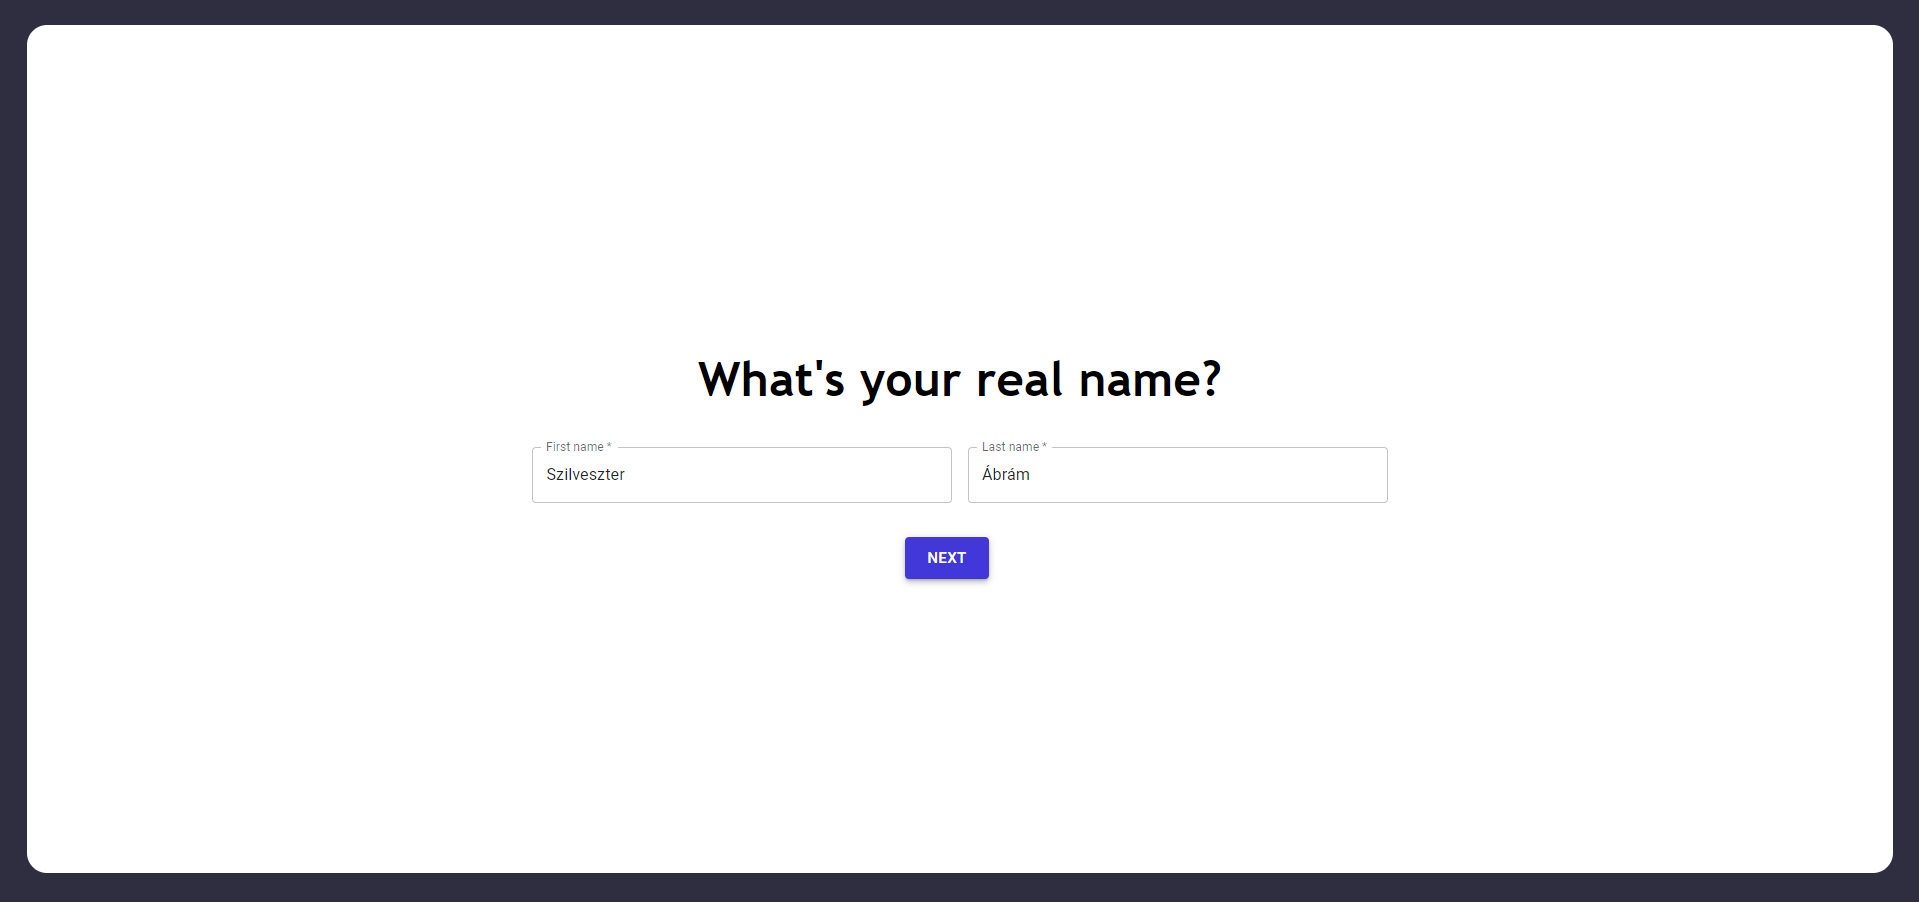
\includegraphics[width=0.5\textwidth]{images/register_1.png}
	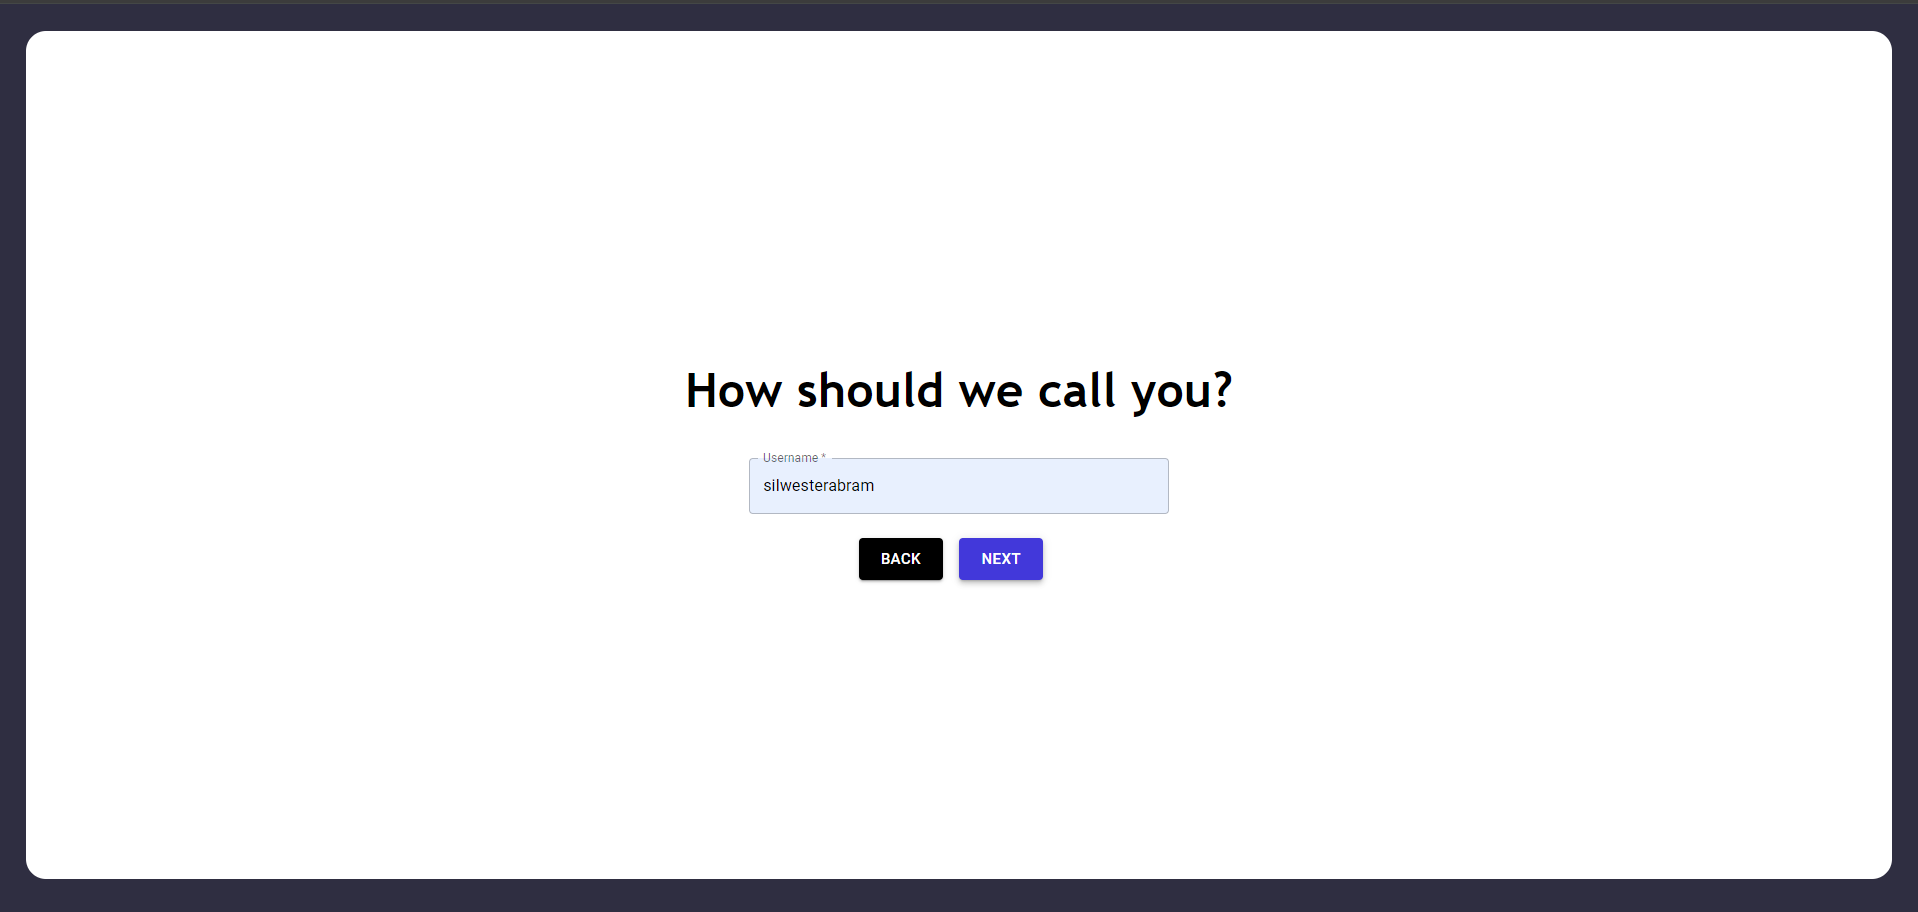
\includegraphics[width=0.5\textwidth]{images/register_2.png}
	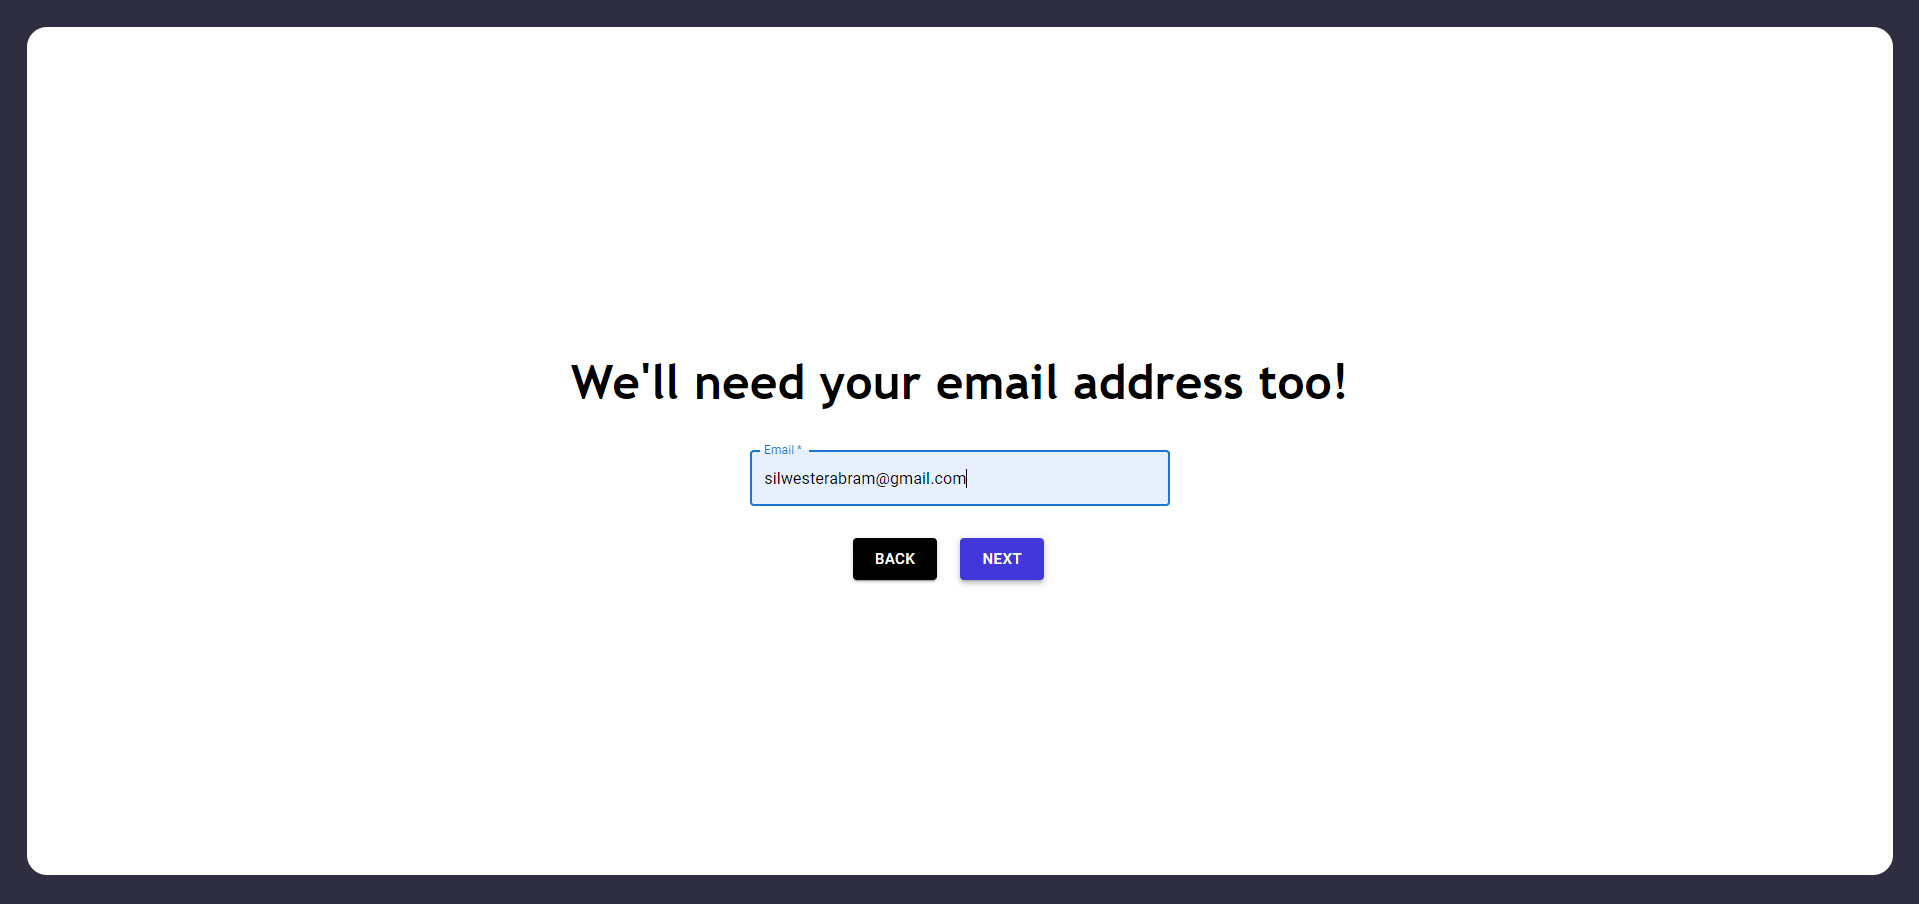
\includegraphics[width=0.5\textwidth]{images/register_3.png}
	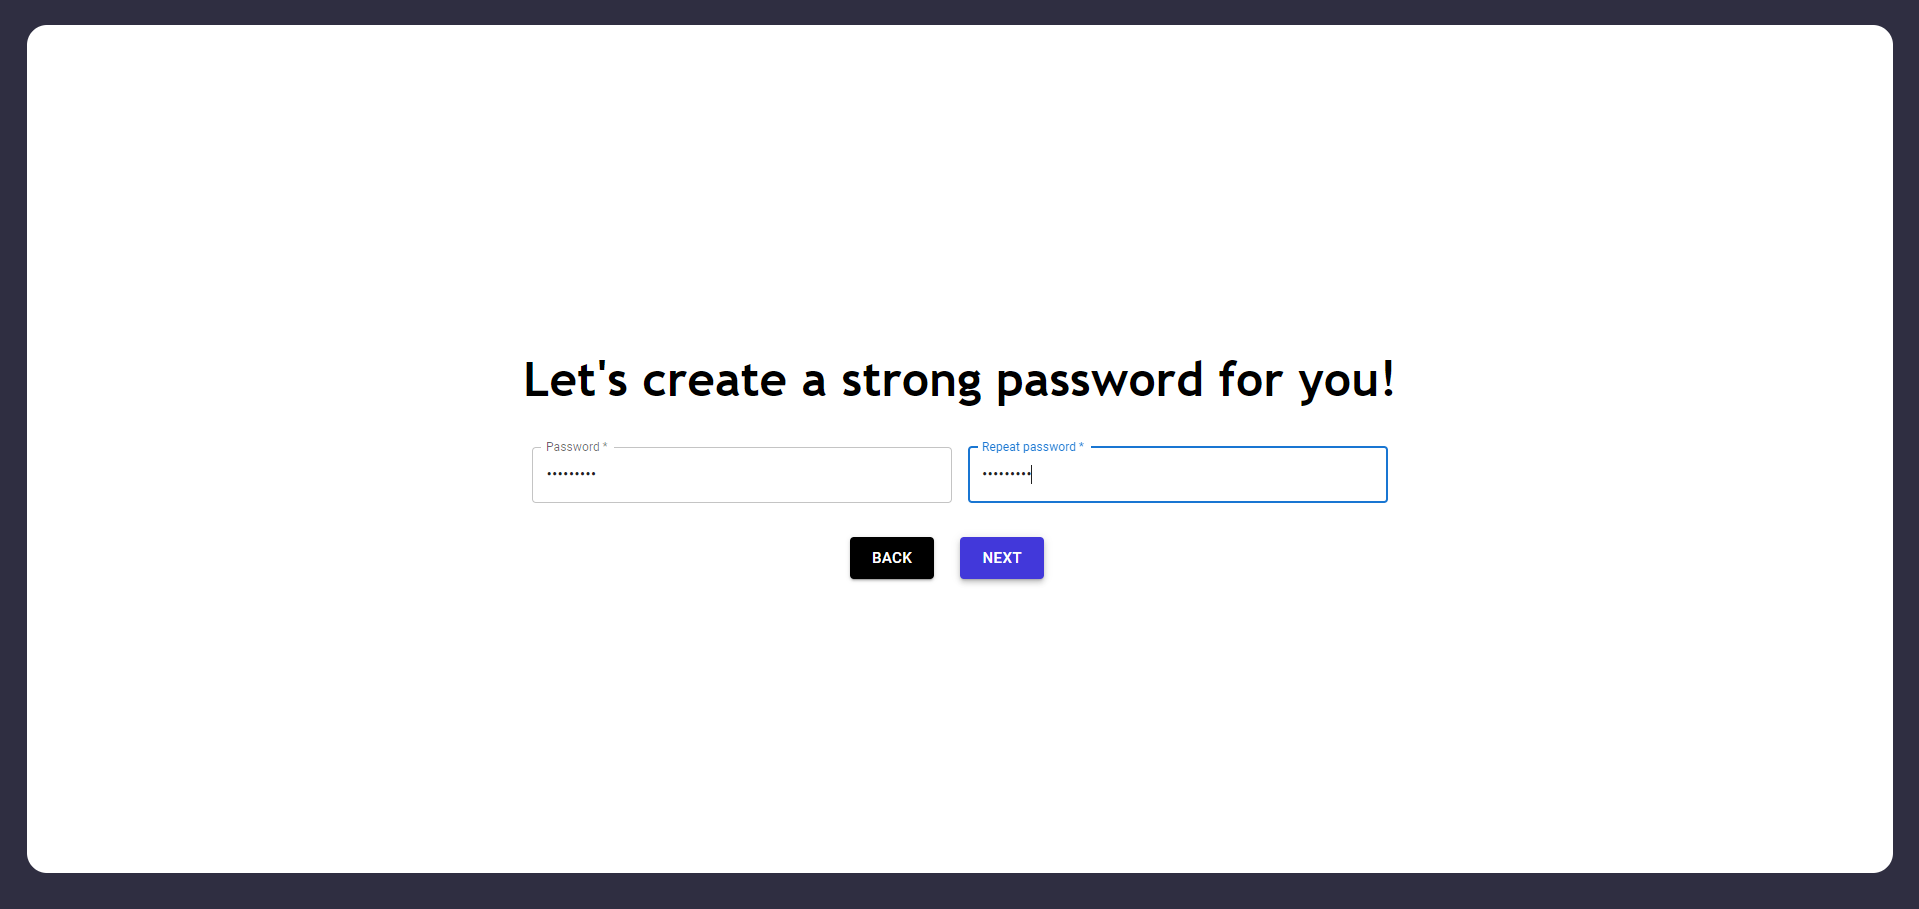
\includegraphics[width=0.5\textwidth]{images/register_4.png}
	\begin{center}
		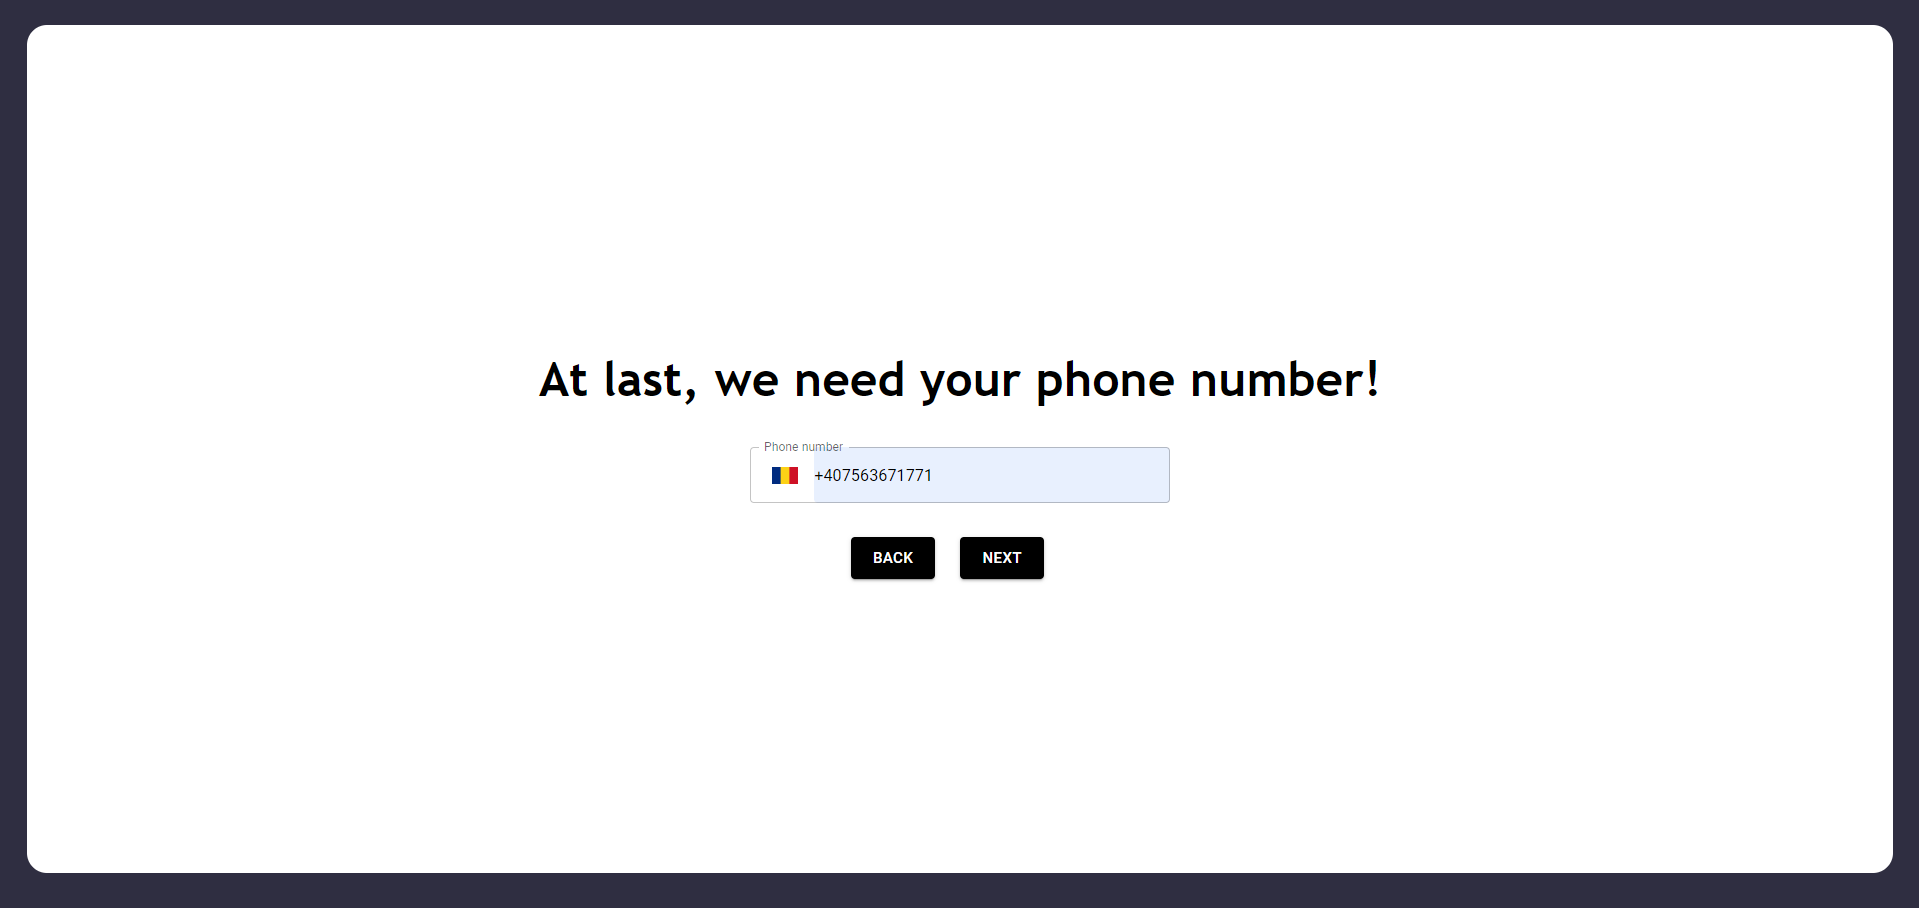
\includegraphics[width=0.5\textwidth]{images/register_5.png}
	\end{center}
	\caption{A regisztrációs folyamat}
	\label{fig:registration_seq}
\end{figure}

\newpage

\section{A profil oldal}

A regisztráció alkalmával megadott információk megtekinthetők a profil oldalon. Itt lehetőség van arra is, hogy a felhasználó megváltoztassa a személyes
információit, illetve profil és borítóképét is. Ez látható a \ref{fig:profile_page}-as ábrán.

\begin{figure}[ht]
	\centering
	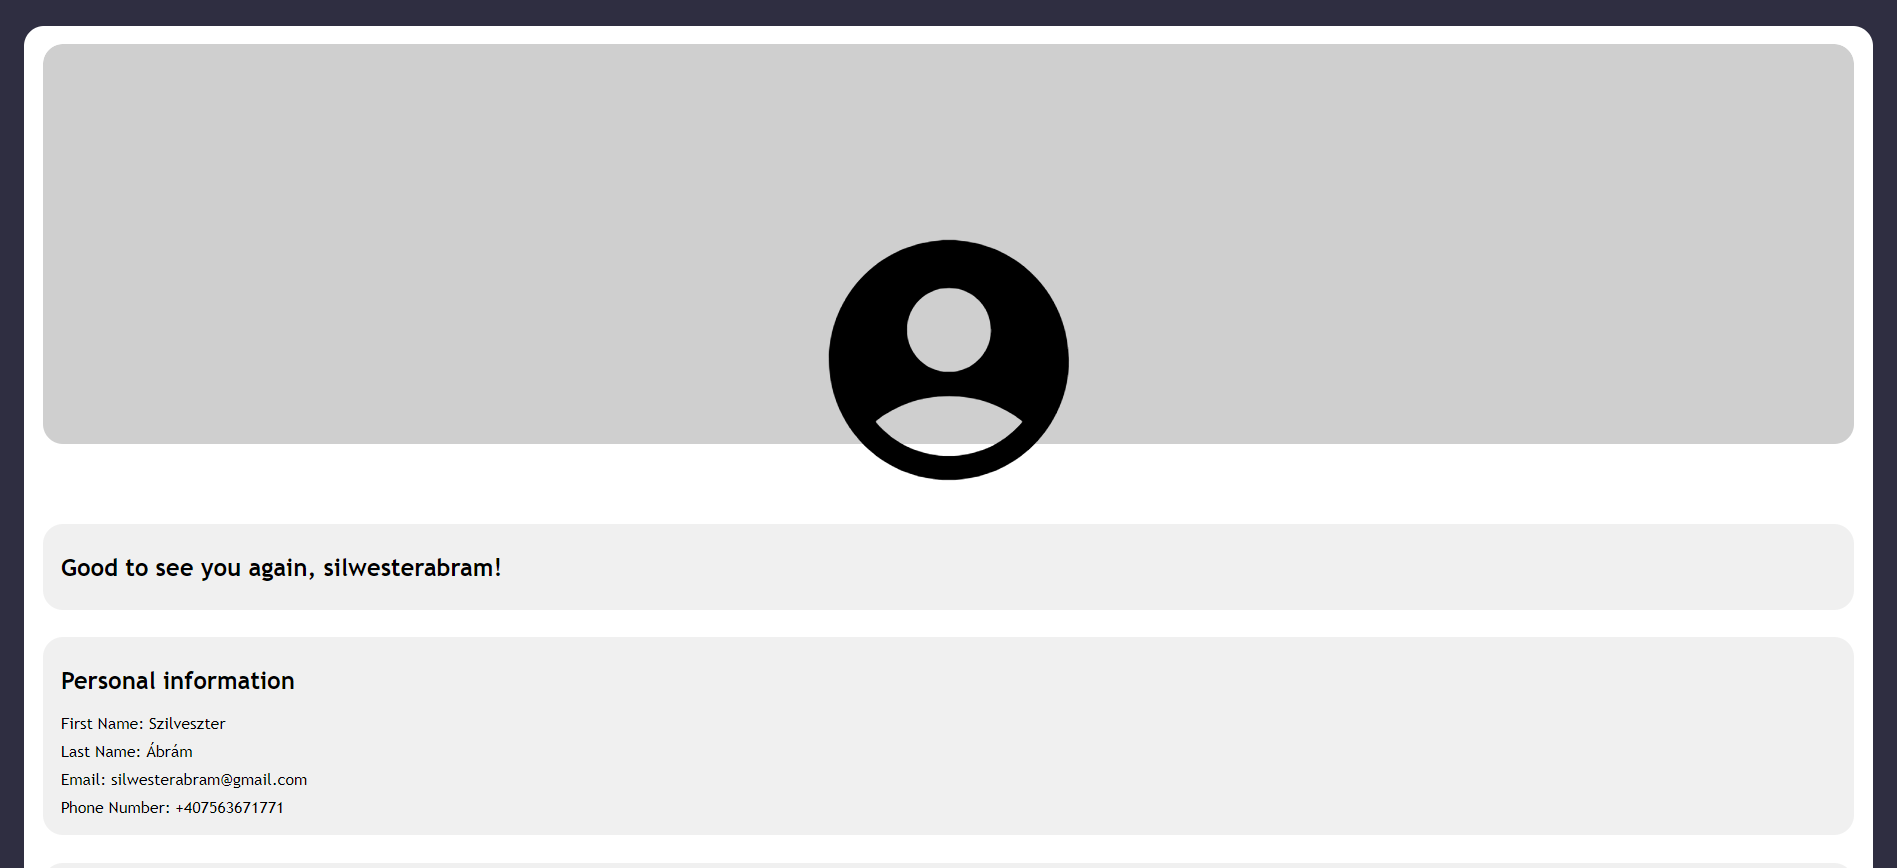
\includegraphics[width=0.6\textwidth]{images/profile_1.png}
	\caption{A profil oldal}
	\label{fig:profile_page}
\end{figure}

A Profil oldalon való ``Edit Profile''-ra való kattintással előhozható egy felület, ahol a felhasználó megváltoztathatja személyes információit,
illetve lehetősége van arra is, hogy profil és borítóképet változtasson, hogy egyéni stílusát tükrözze a felületen. Ez látható a 
\ref{fig:profile_edit_page}-es ábrán.

\begin{figure}[h]
		\centering
		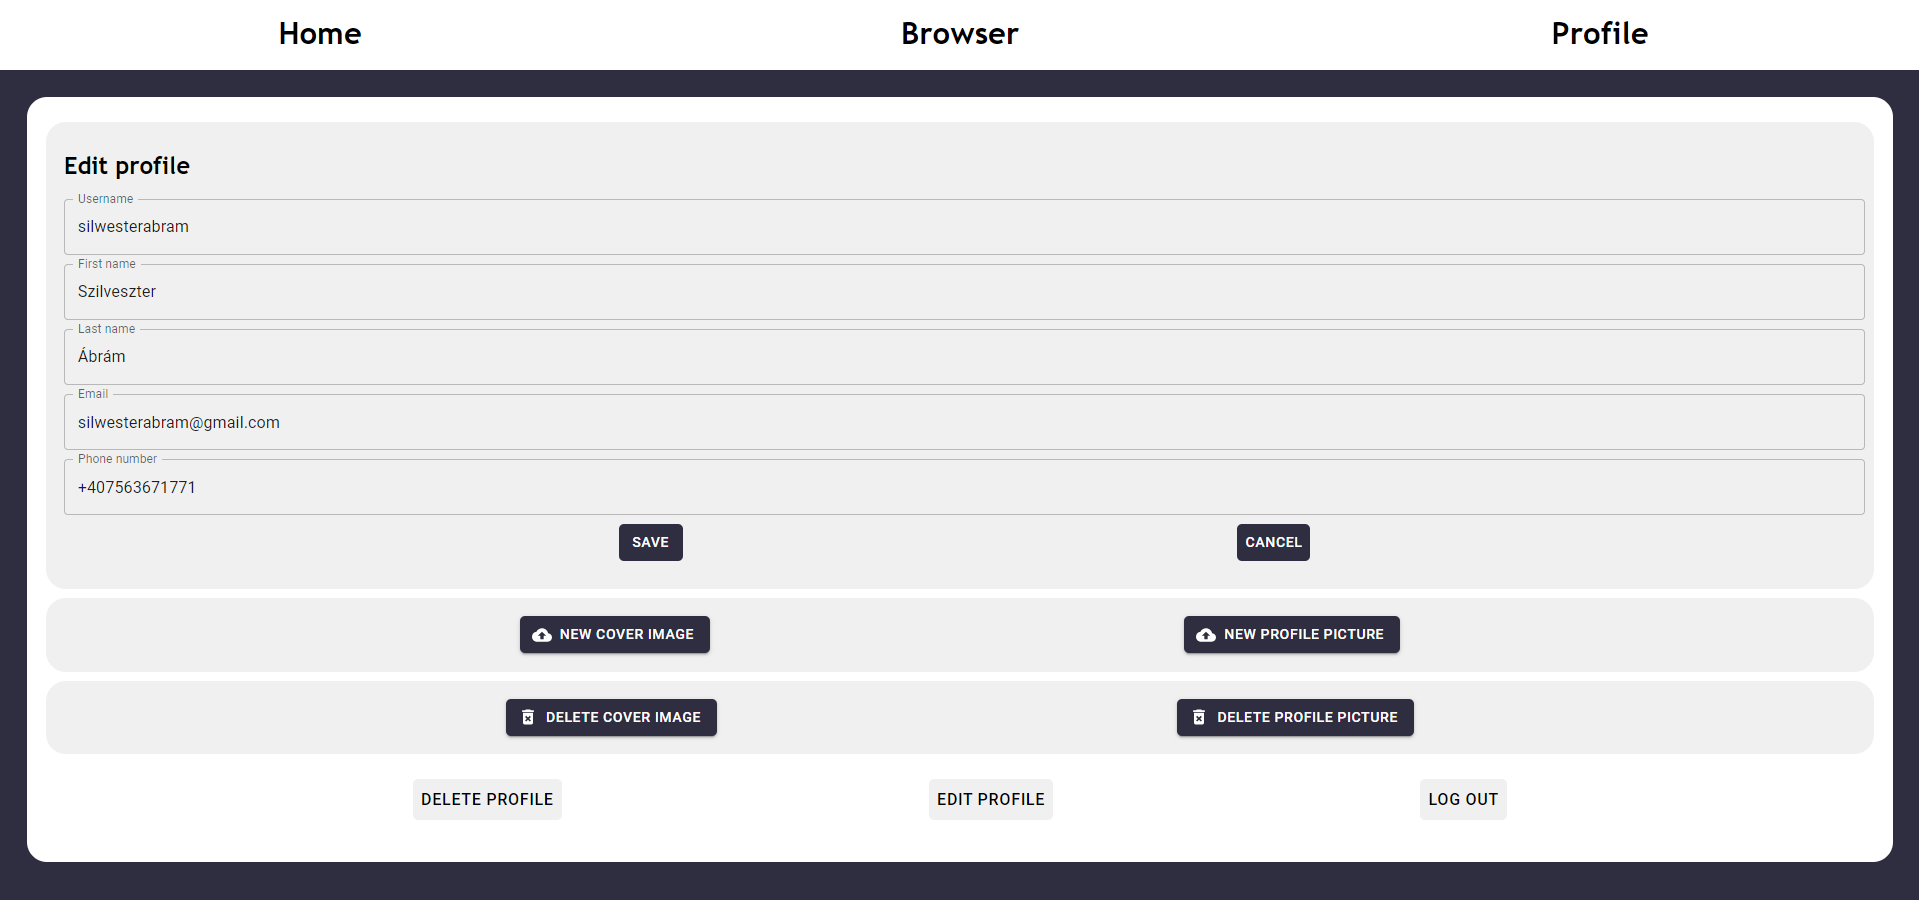
\includegraphics[width=0.6\textwidth]{images/profile_edit.png}
		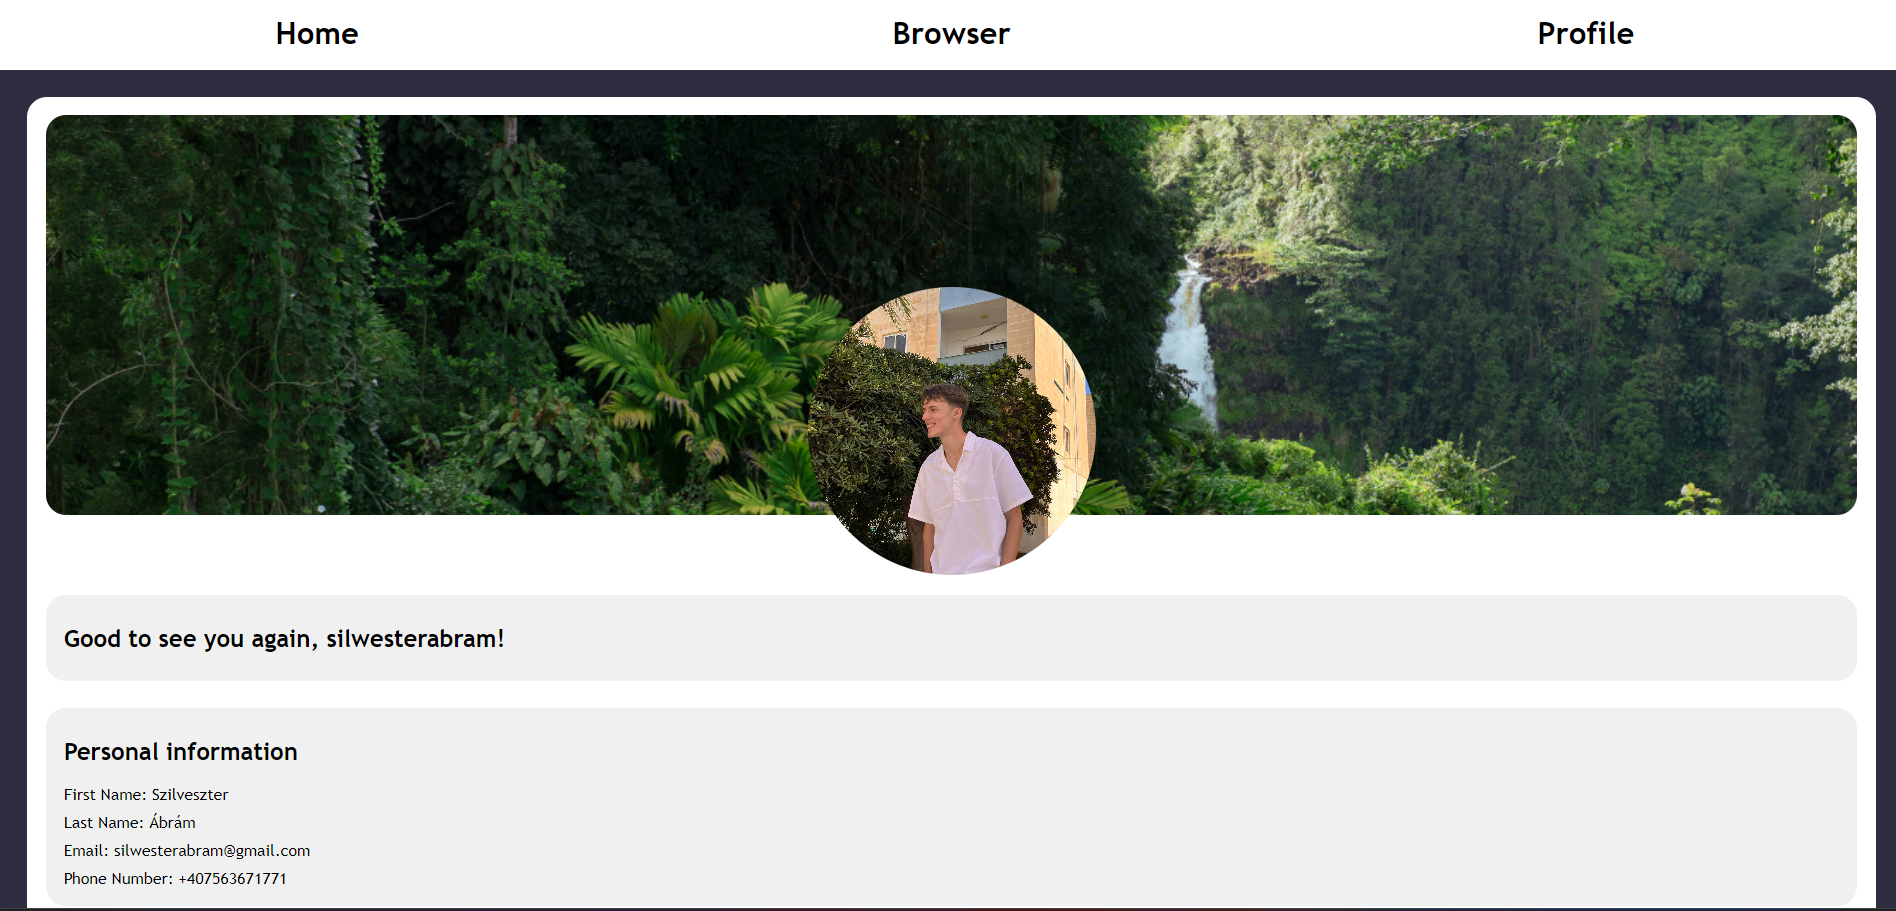
\includegraphics[width=0.6\textwidth]{images/profile_2.png}
	\caption{A profil szerkesztése}
	\label{fig:profile_edit_page}
\end{figure}

A továbbiakban lehetőségünk van a felhasználónk törlésére is. A ``Delete Profile'' gomb megnyomásával előhozható egy prompt, 
amit ha továbbra is megerősítünk, akkor egyszerűen törölhetjük a felhasználónkat, s minden vele kapcsolatos információt, eseményt. [\ref{fig:delete_profile}-ös ábra]

\begin{figure}
	\centering
	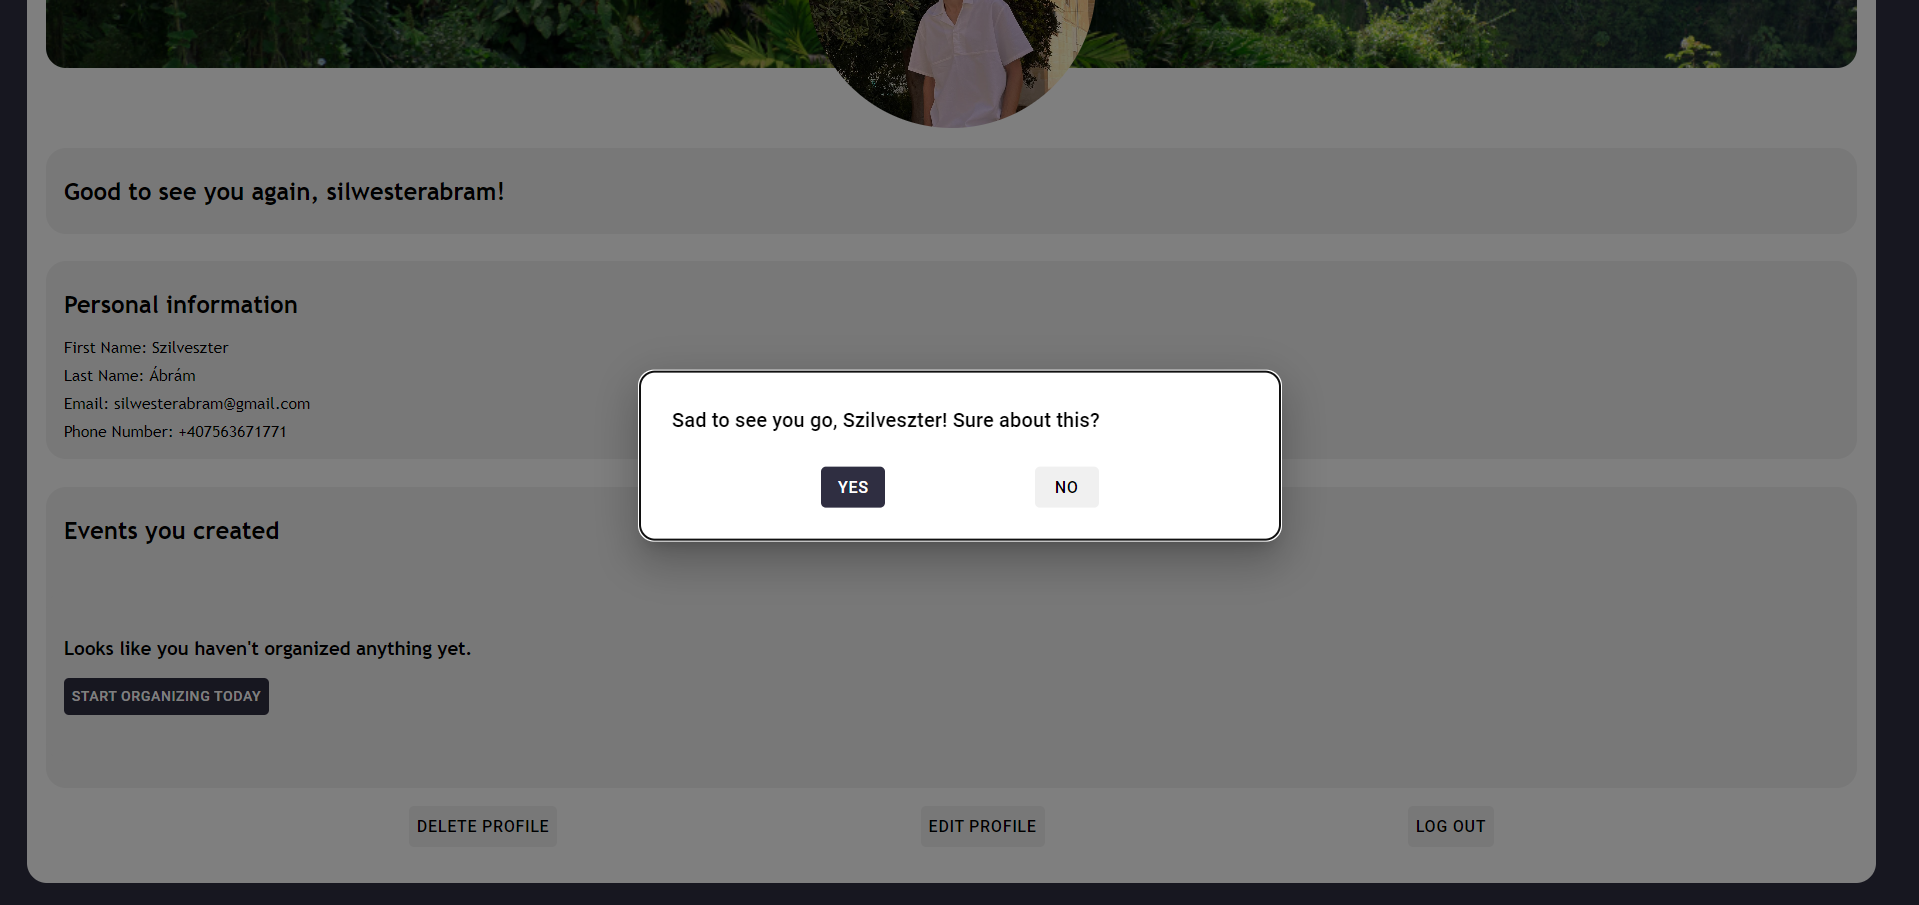
\includegraphics[width=0.7\textwidth]{images/delete_profile.png}
	\caption{A profil törlése}
	\label{fig:delete_profile}
\end{figure}

Az oldal listázza az általunk szervezett sporteseményeket is. Mivel egy újonnan létrehozott felhasználónk van, még nem hoztunk létre egyetlen
sporteseményt sem, így a lista üres. Ilyenkor ezt jelzi nekünk az oldal, illetve ennek megfelelően jelenít meg egy gombot, amivel átirányít
bennünket arra a felületre, ahol létrehozhatunk új sporteseményeket. [\ref{fig:profile_page_2}-os ábra]

\begin{figure}[h]
	\centering
	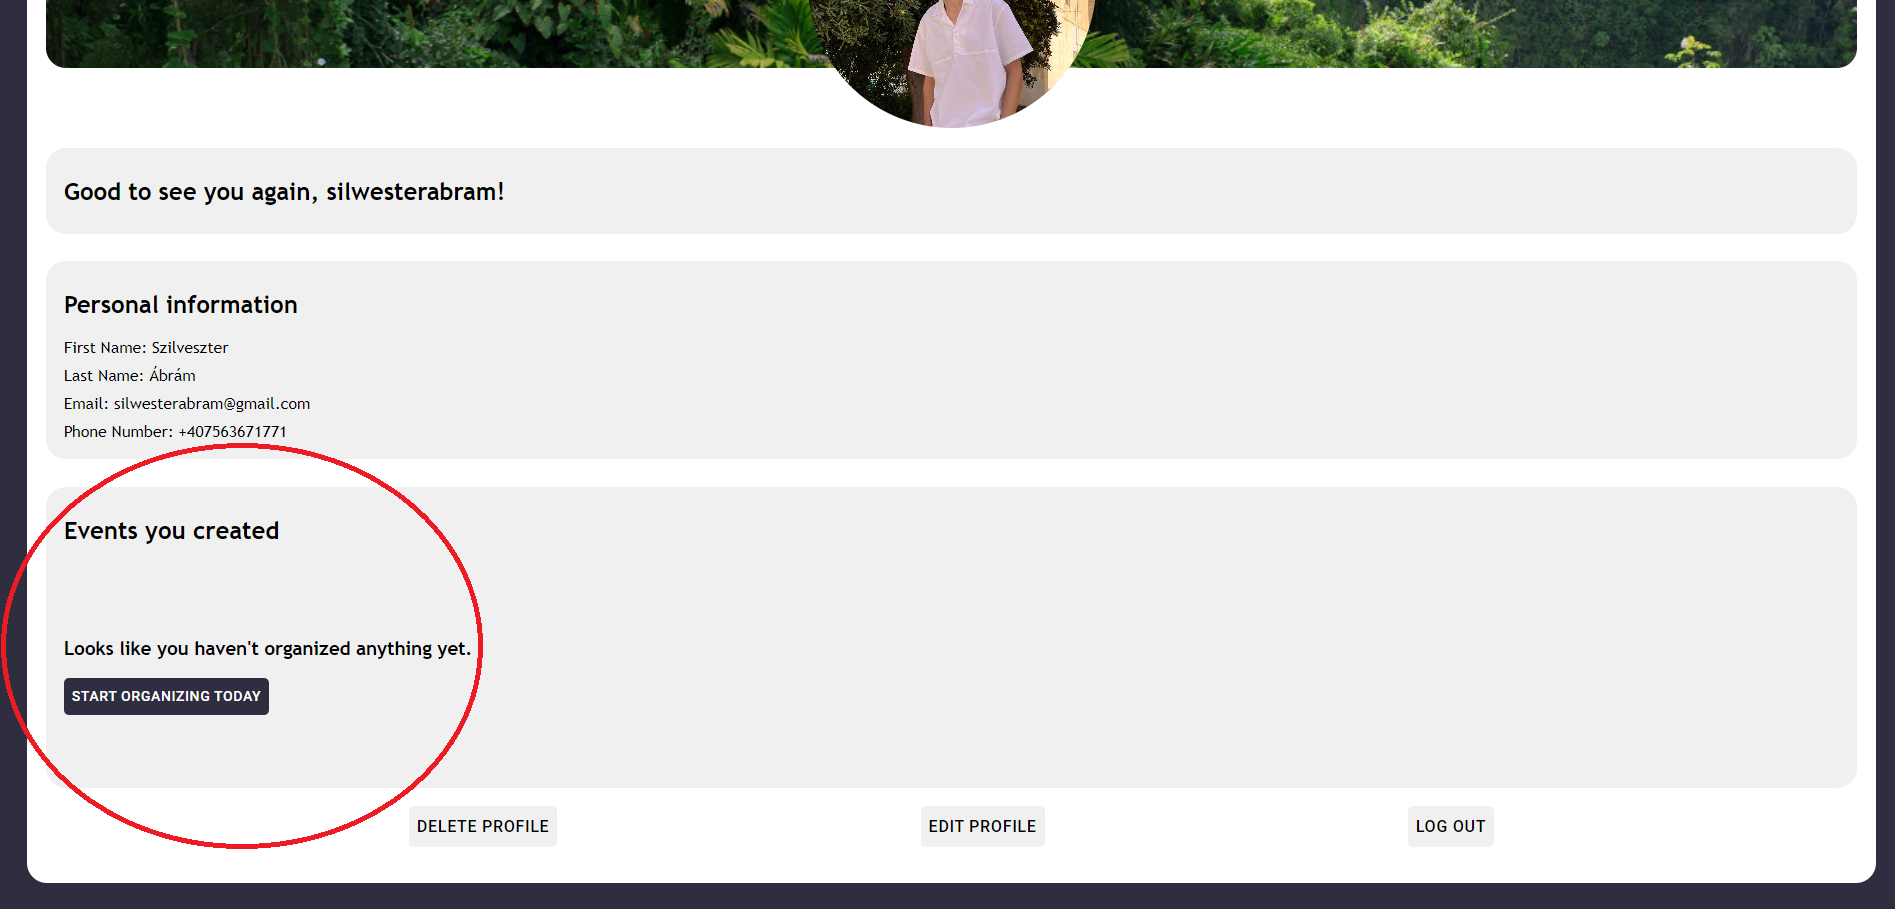
\includegraphics[width=0.7\textwidth]{images/events_by_you_profile.png}
	\caption{Általunk szervezett sportesemények listázása a profil oldalon}
	\label{fig:profile_page_2}
\end{figure}

\section{A sportesemény böngésző}

A sportesemény böngésző, azaz a ``Browser'' oldal két fő részre osztható. A ``See what others are up to'' fül alatt listázhatjuk az összes
létrehozott sporteseményt, míg a ``Create a new event'' lehetőséget ad arra, hogy létrehozhassuk egy új, saját eseményt.
Ez látható a \ref{fig:browser_page}-es ábrán is.

\newpage

\begin{figure}[ht]
	\centering
	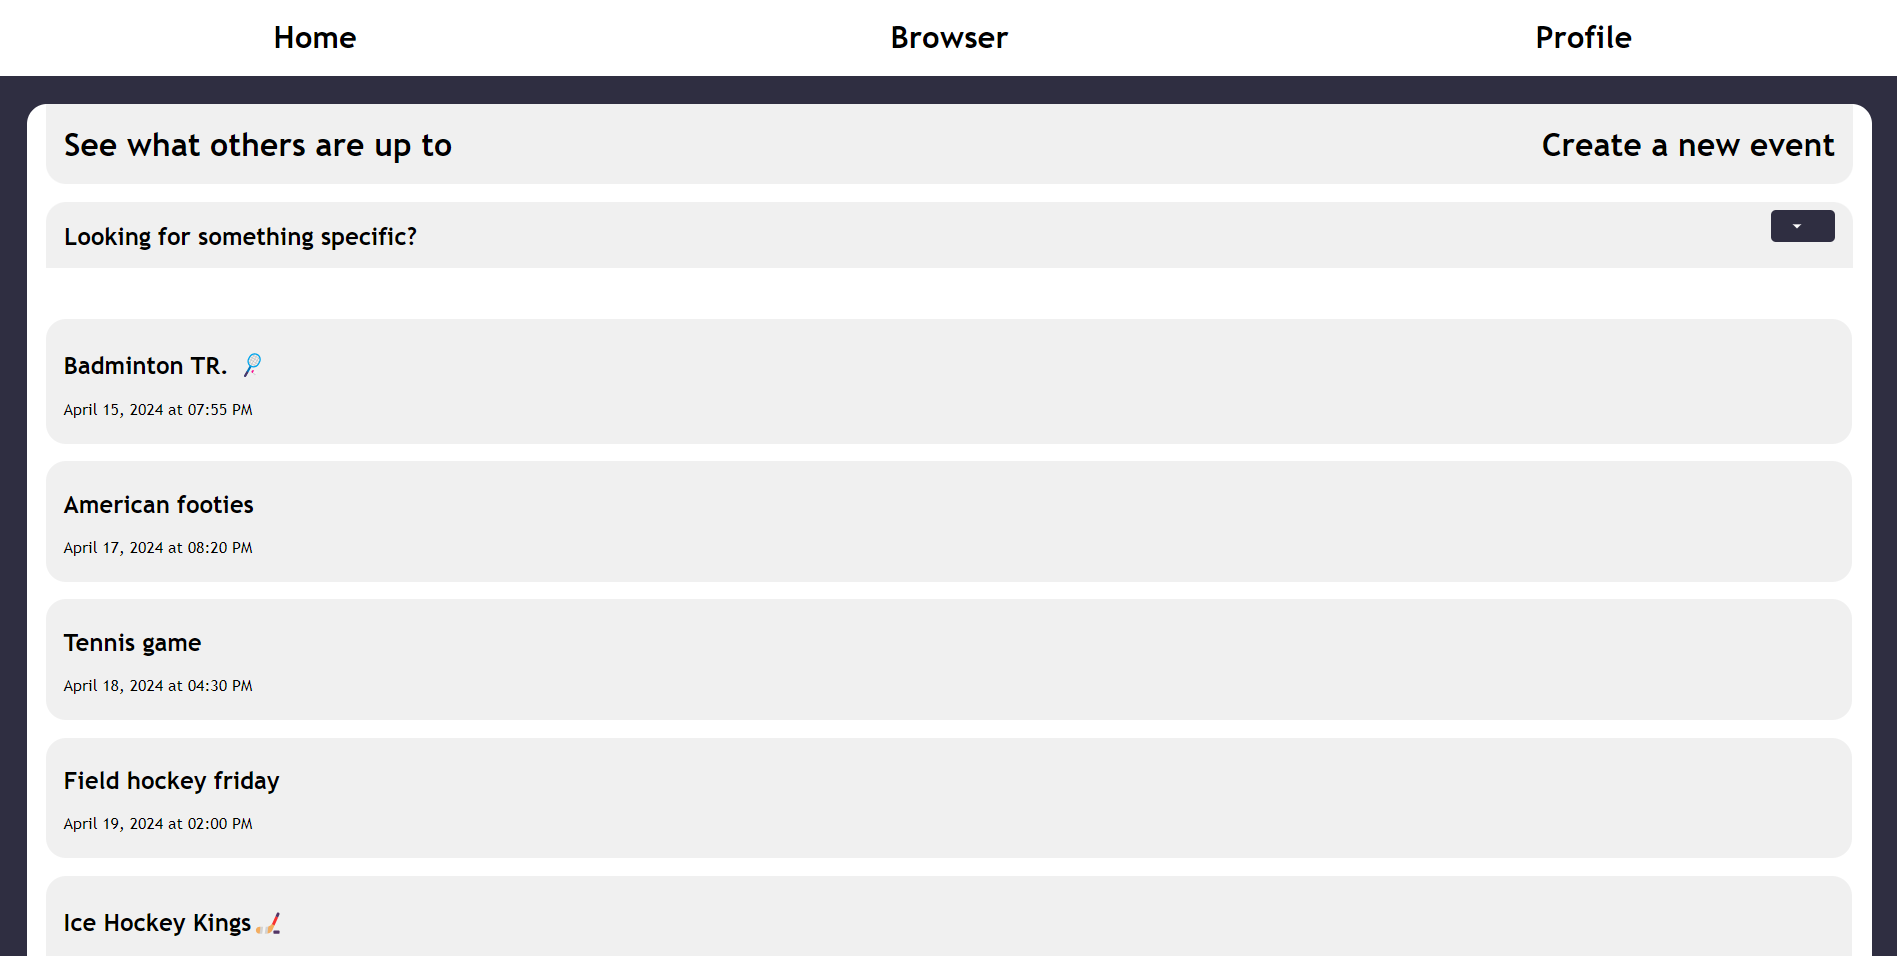
\includegraphics[width=0.7\textwidth]{images/browser_page.png}
	\caption{A sportesemény böngésző}
	\label{fig:browser_page}
\end{figure}

Egy új esemény létrehozása során egy egyszerű űrlapot kell kitöltenie a felhasználónak. Itt meglévő sportok közül választhat, az esemény témájaként.
Megfelelő információk, sport, dátum és résztvevőszám megadása után a ``Submit'' gombra kattintás hozhatja létre az általa kívánt eseményt.
Ez a folyamat látható a \ref{fig:create_event}-as ábrán. Az esemény sikeres létrehozása után megfigyelhetjük, hogy az esemény megjelenik a sportesemény böngészőben is. Itt rákattintás segítségével előhozható
egy részletesebb nézet. [\ref{fig:new_event_created}-es ábra]

\begin{figure}[h]
	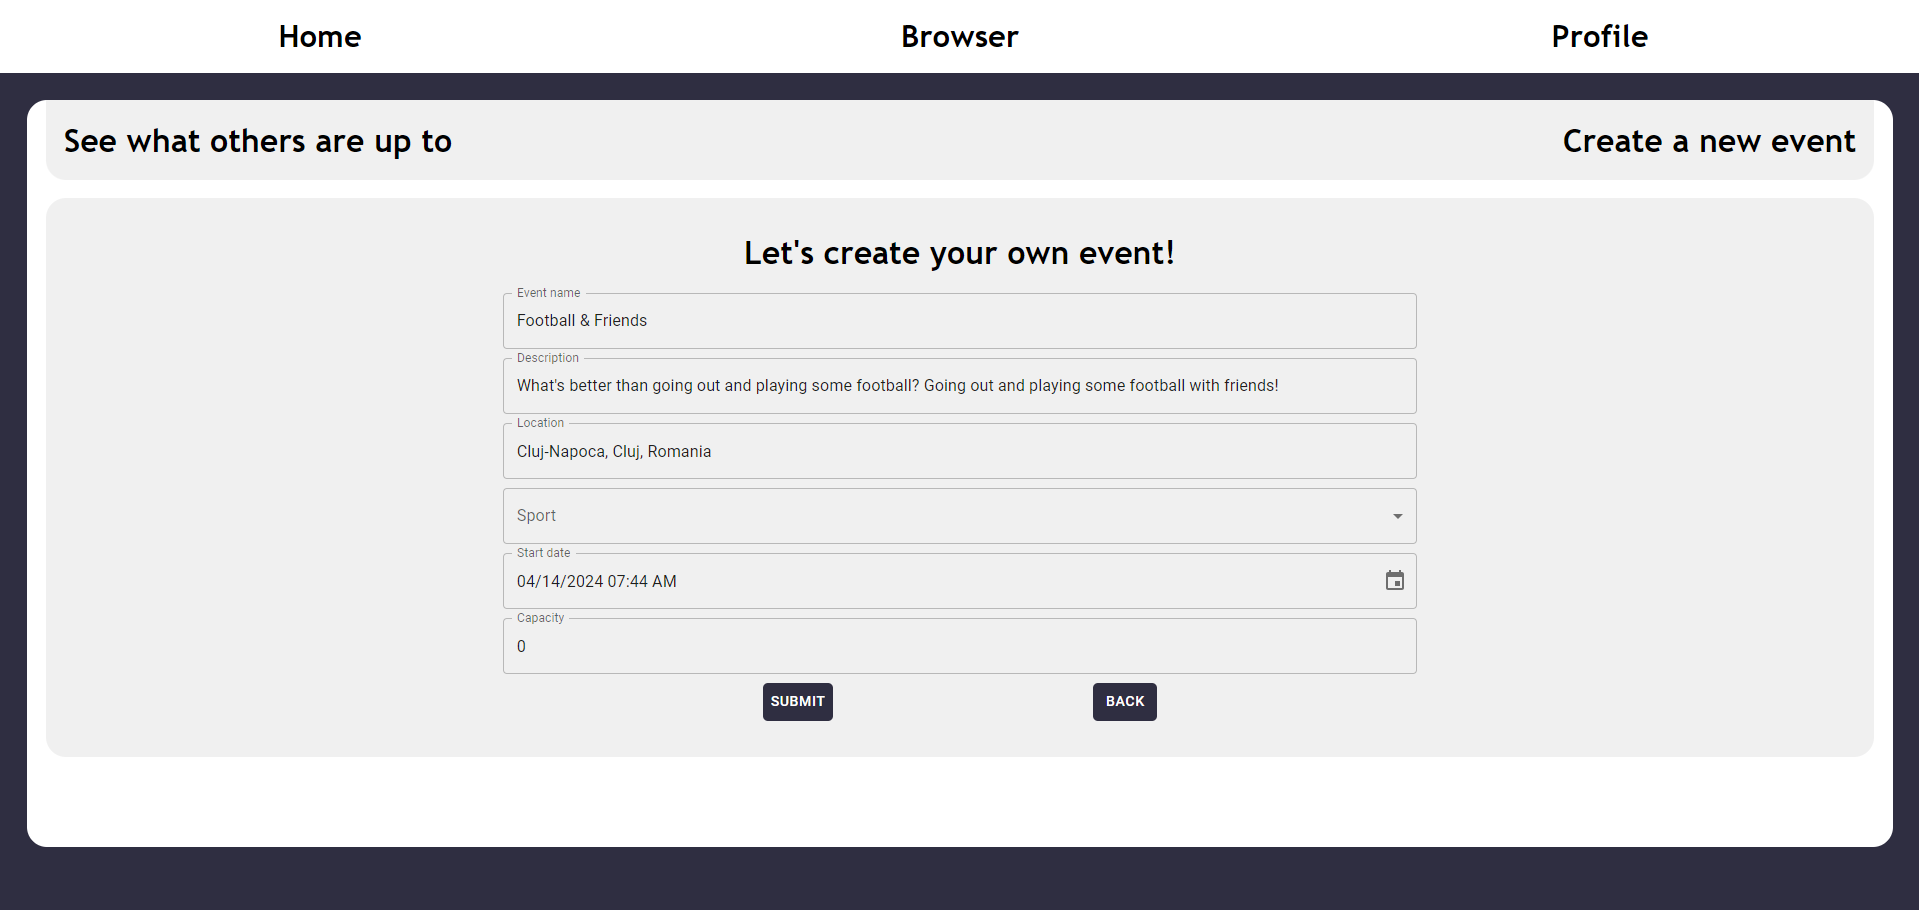
\includegraphics[width=0.5\textwidth]{images/create_event_1.png}
	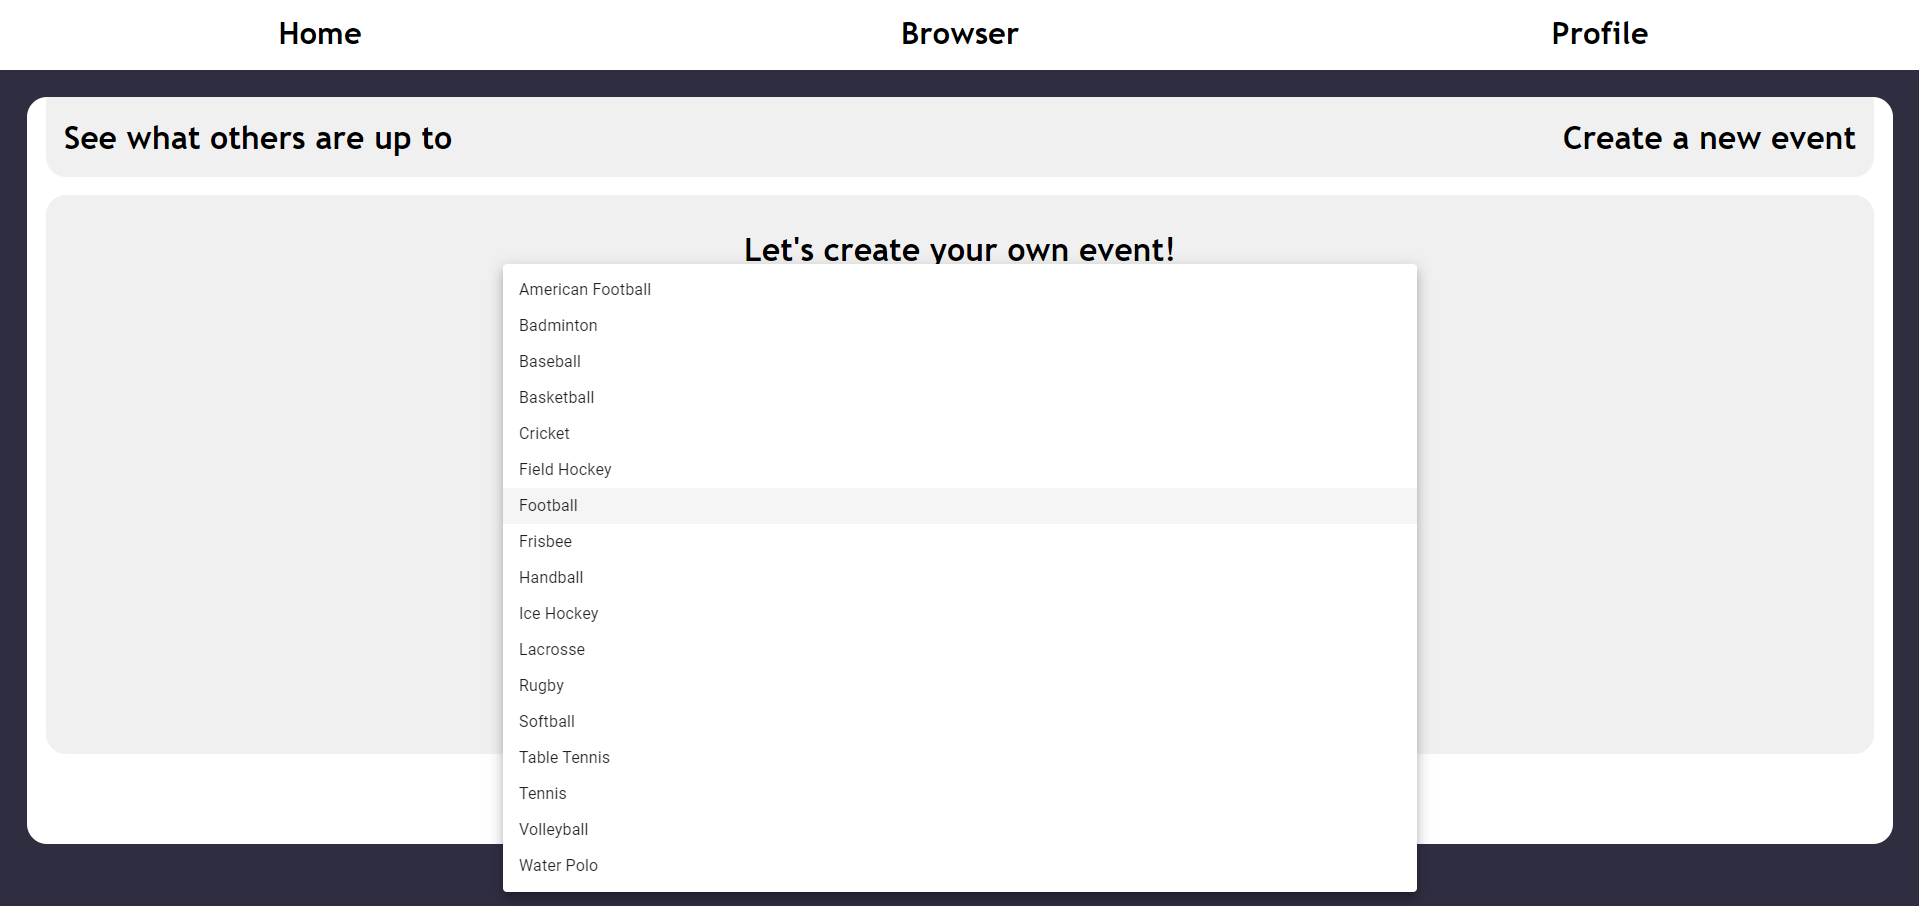
\includegraphics[width=0.5\textwidth]{images/create_event_2.png}
	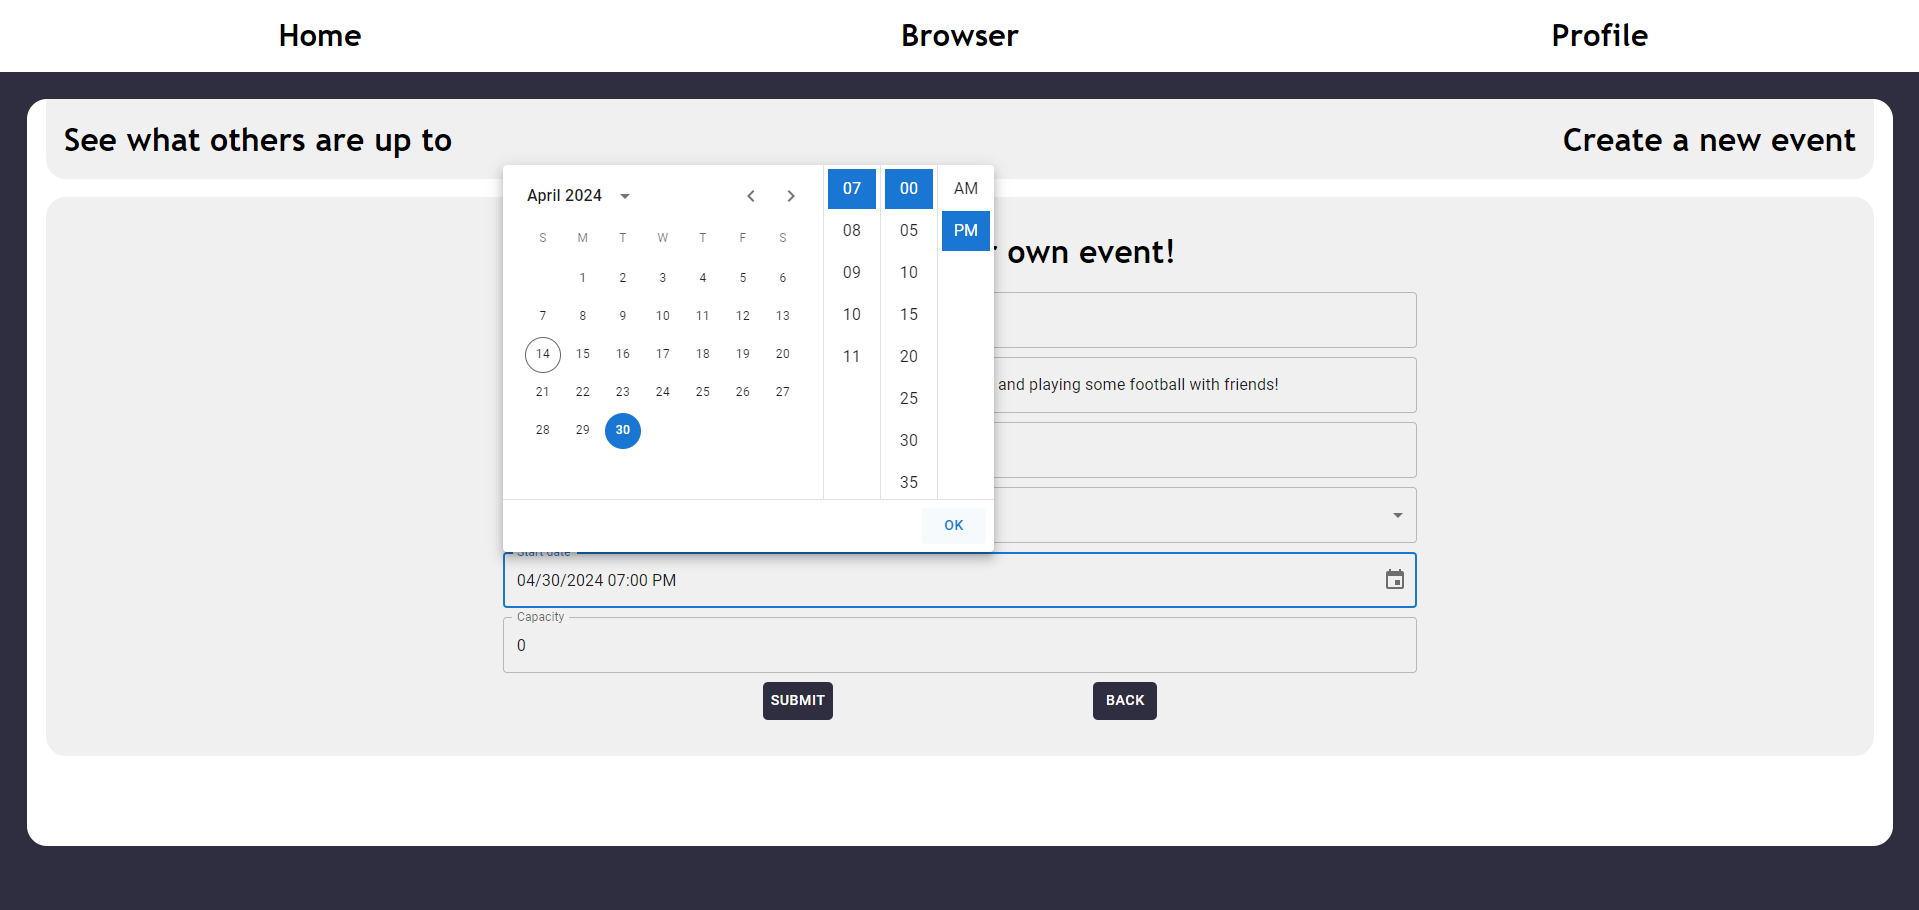
\includegraphics[width=0.5\textwidth]{images/create_event_3.png}
	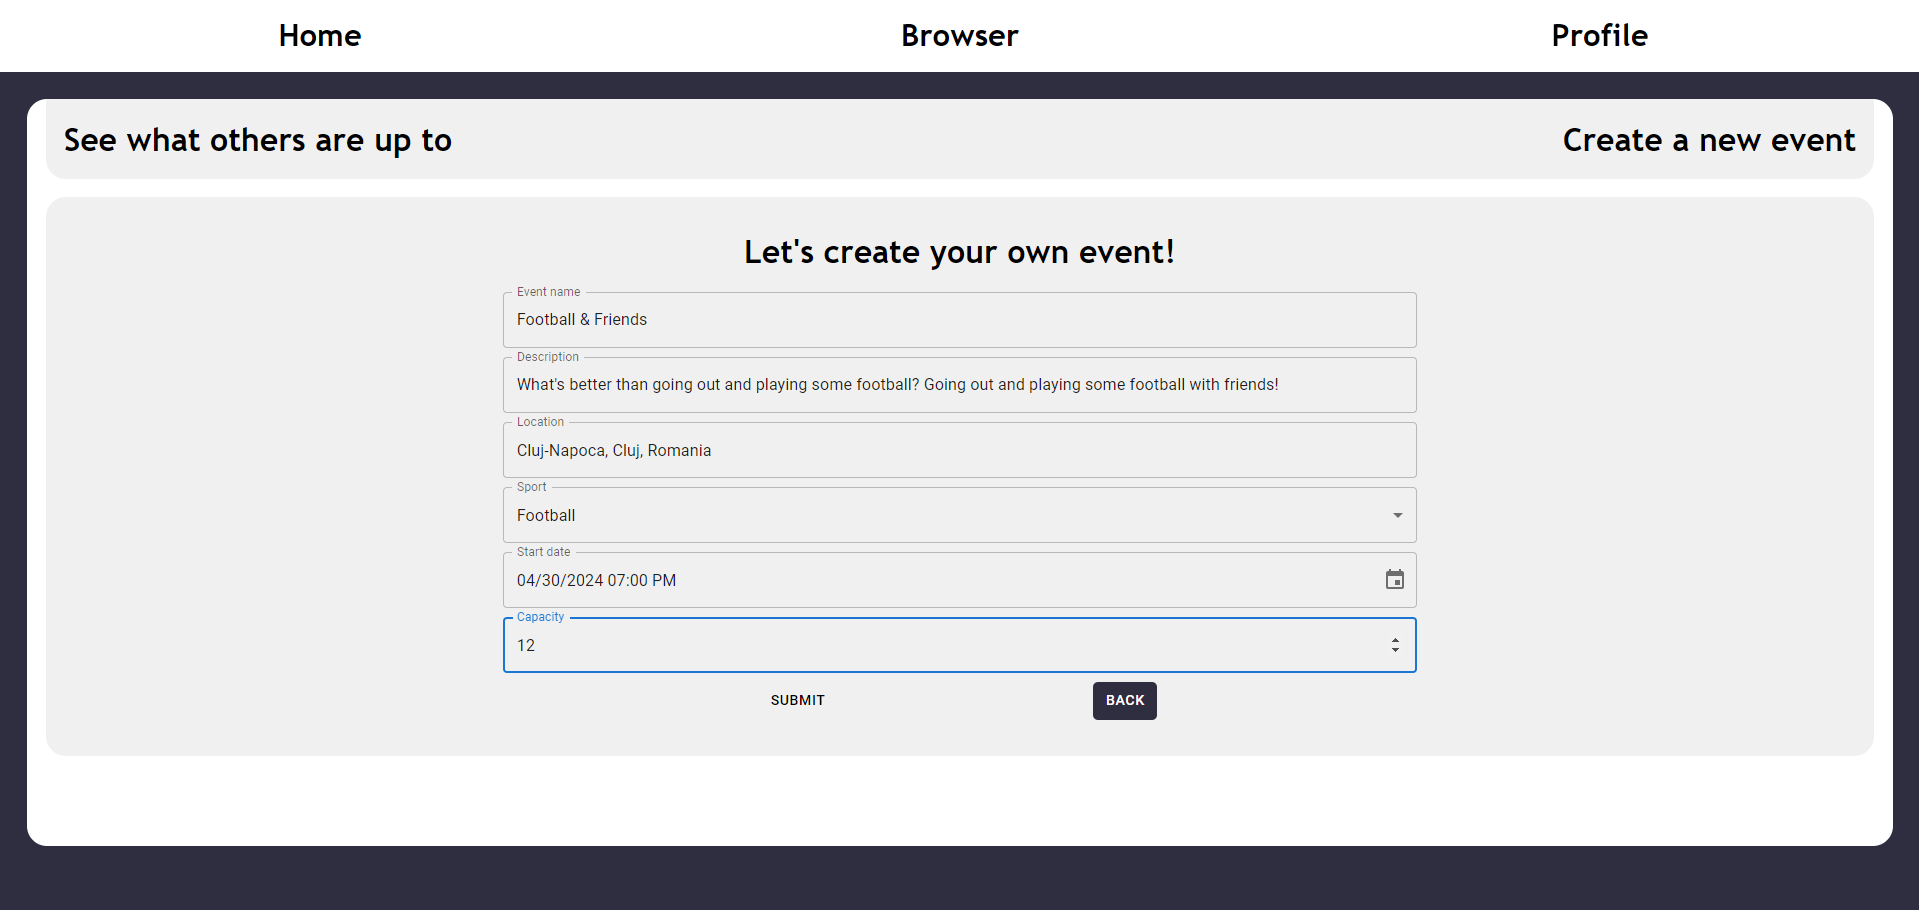
\includegraphics[width=0.5\textwidth]{images/create_event_4.png}
	\caption{Esemény létrehozása}
	\label{fig:create_event}
\end{figure}

\newpage

\begin{figure}[ht]
	\centering
	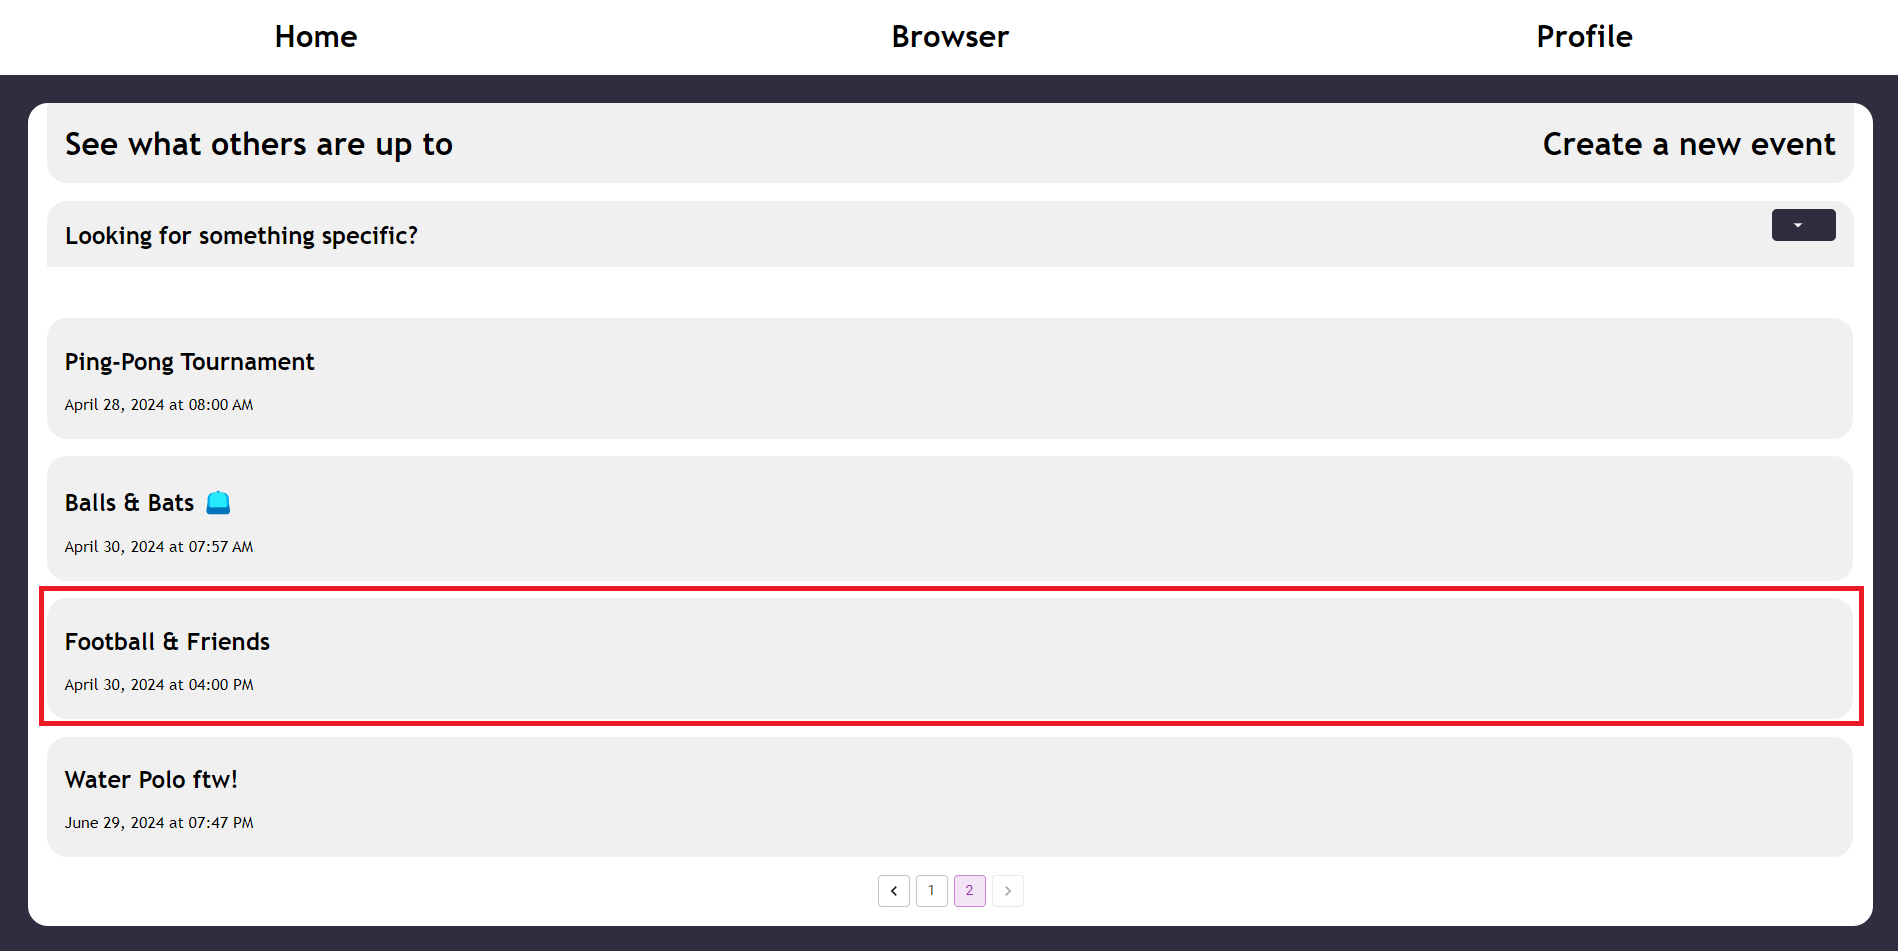
\includegraphics[width=0.7\textwidth]{images/new_event_created.png}
	\caption{Az újonnan létrehozott esemény a sportesemény böngészőben}
	\label{fig:new_event_created}
\end{figure}

Az esemény részletes megjelenítésében látható minden általunk megadott információt. Az eseméy azt is mutatja, hogy ki az esemény szervezője. A szerző nevére
kattintva megtekinthető egy rövid leírás a szervező profiljáról. Ez látható a \ref{fig:event_creator}-es ábrán is.

\begin{figure}[h]
	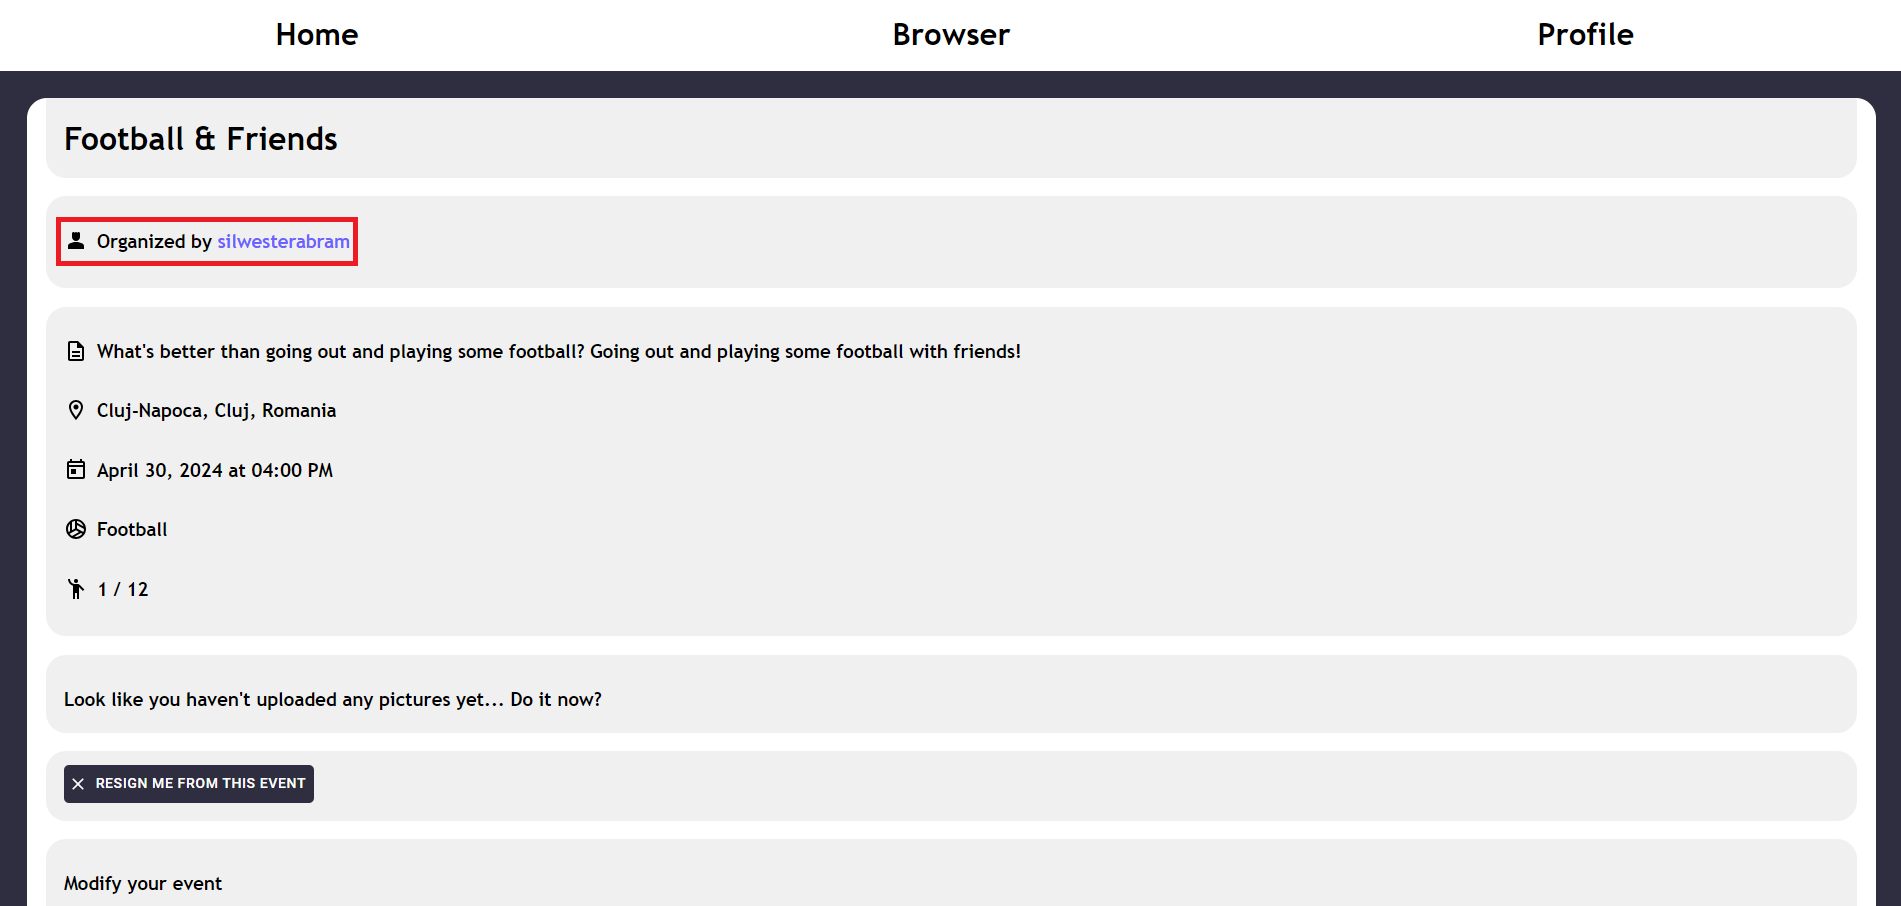
\includegraphics[width=0.5\textwidth]{images/sports_event_creator.png}
	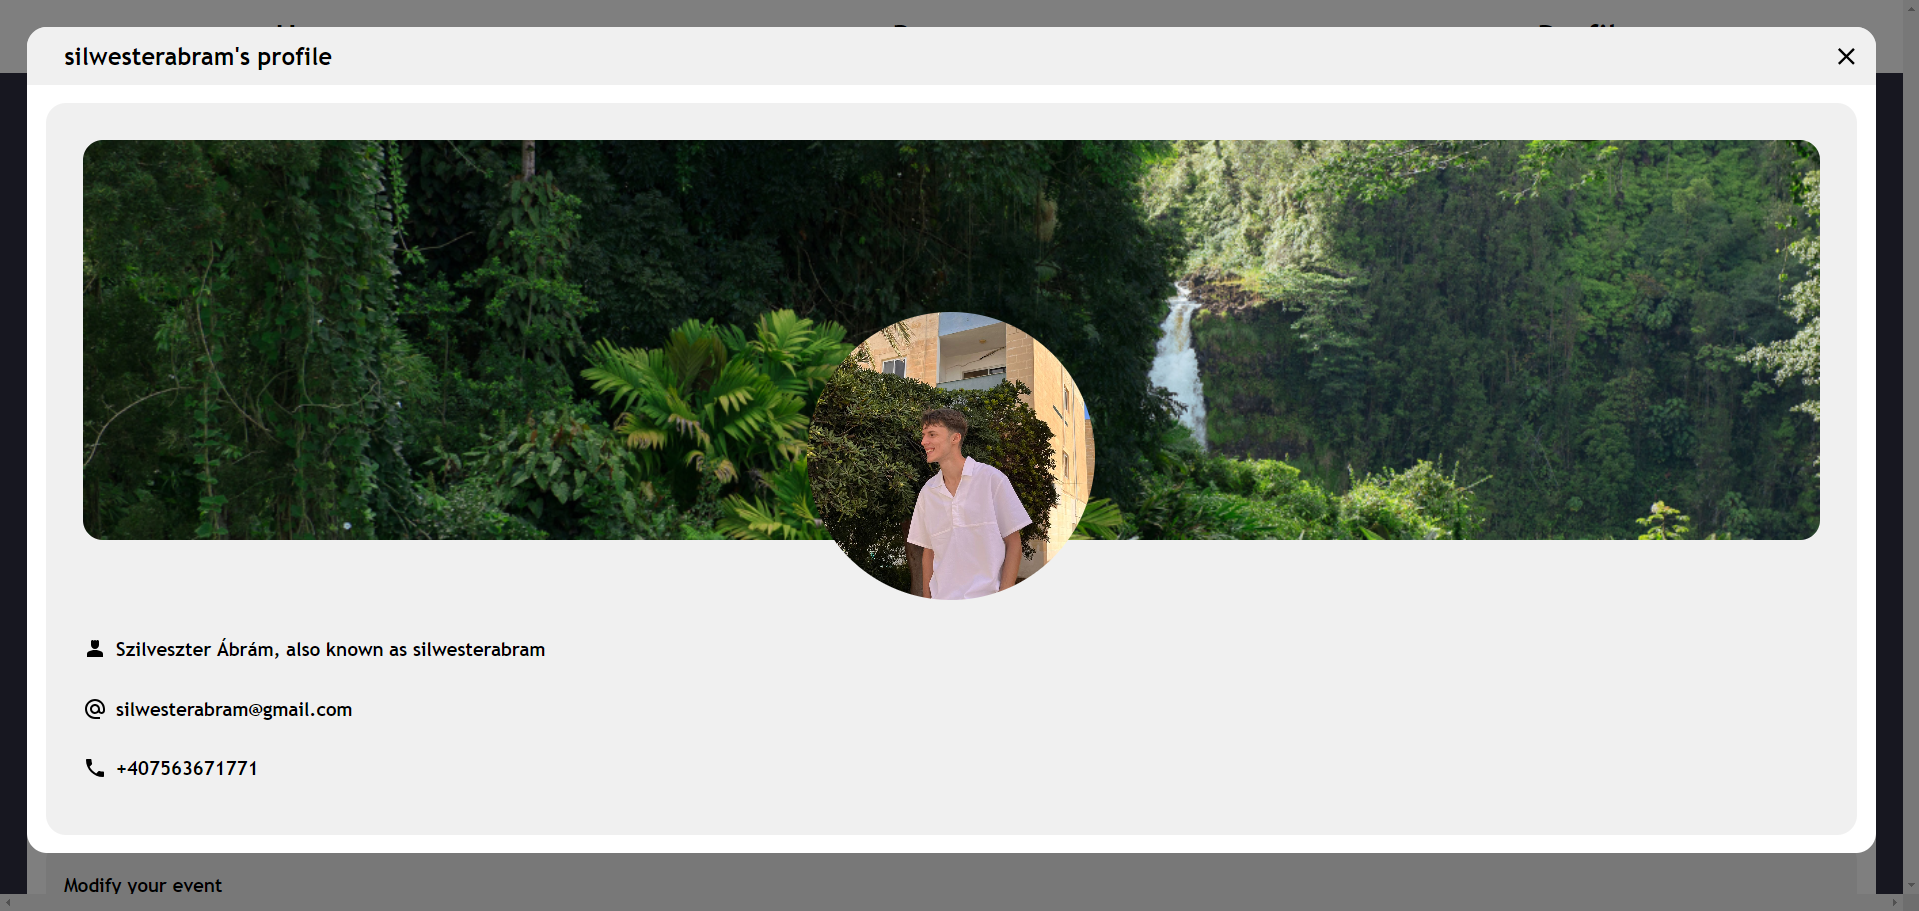
\includegraphics[width=0.5\textwidth]{images/sports_event_creator_profile_view.png}
	\caption{Az esemény szervezőjének megjelenítése}
	\label{fig:event_creator}
\end{figure}

Egy esemény létrehozásakor az esemény szervezője automatikusan feliratkozik erre. Amennyiben ezt vissza szeretné vonni, a
``Resign me from this event'' gomb segítségével megteheti. Ilyenkor megfigyelhető, hogy az eseményre jelentkezett egyének száma egyel csökken.
Ez megfigyelhető a \ref{fig:resign_from_event}-es ábrán.

\begin{figure}[h]
	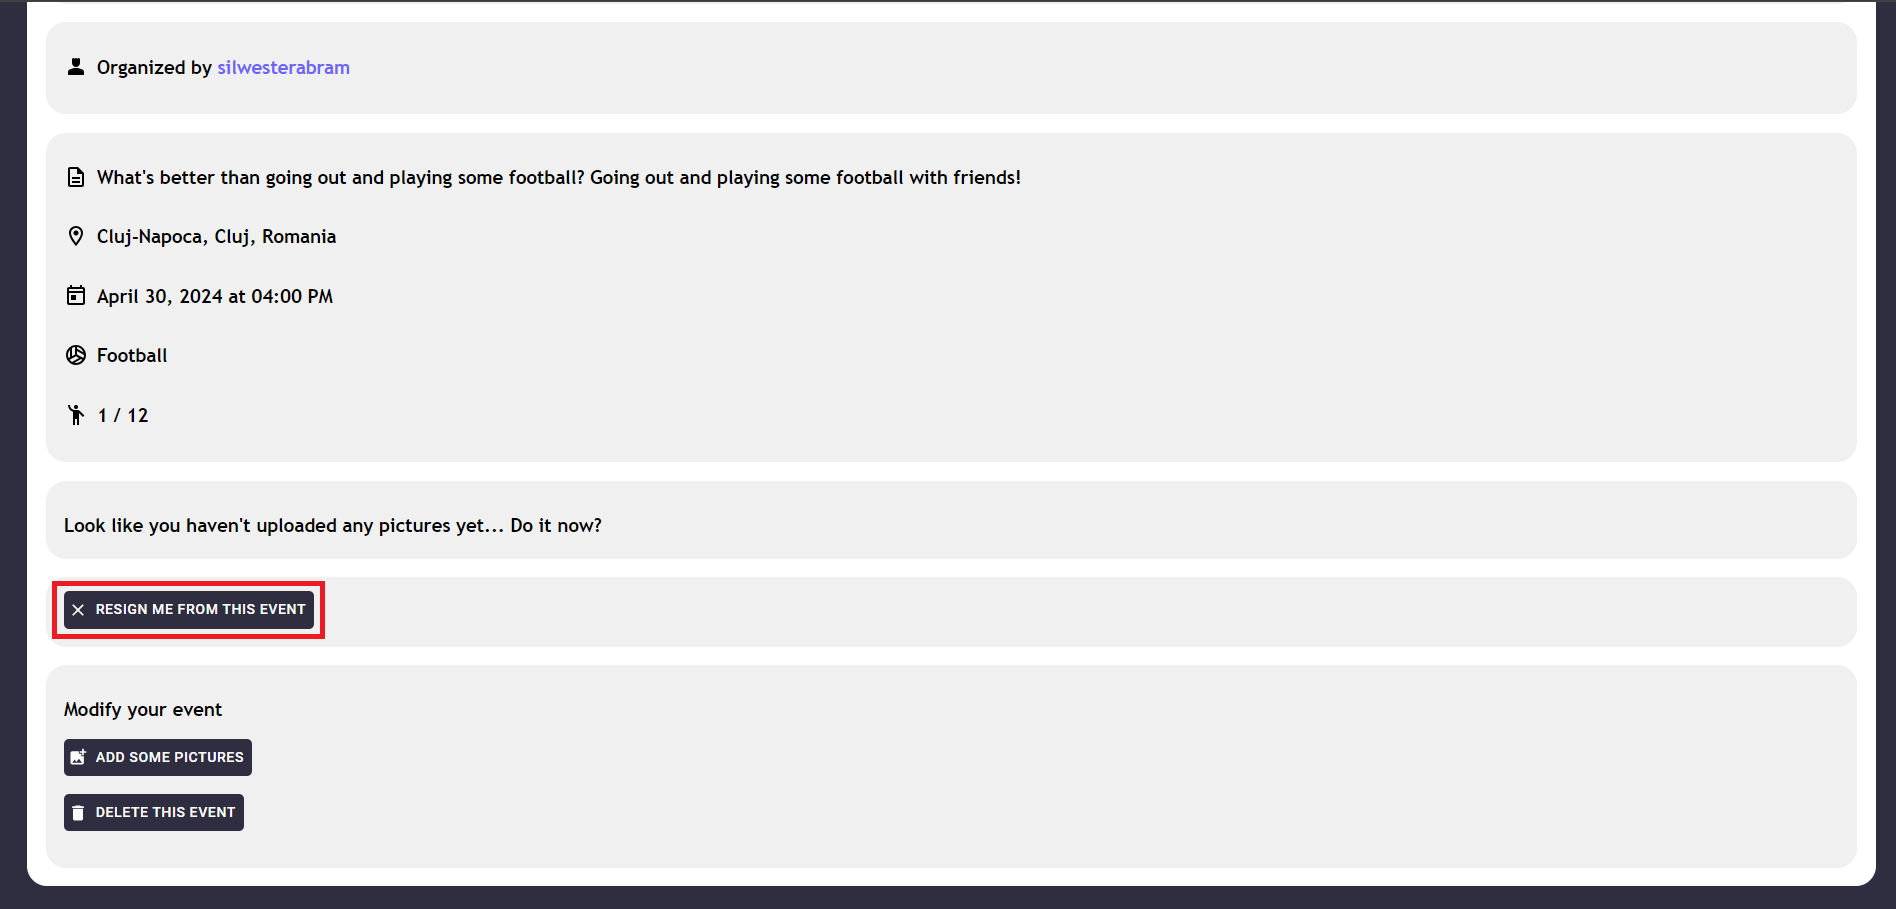
\includegraphics[width=0.5\textwidth]{images/resign_from_event_1.png}
	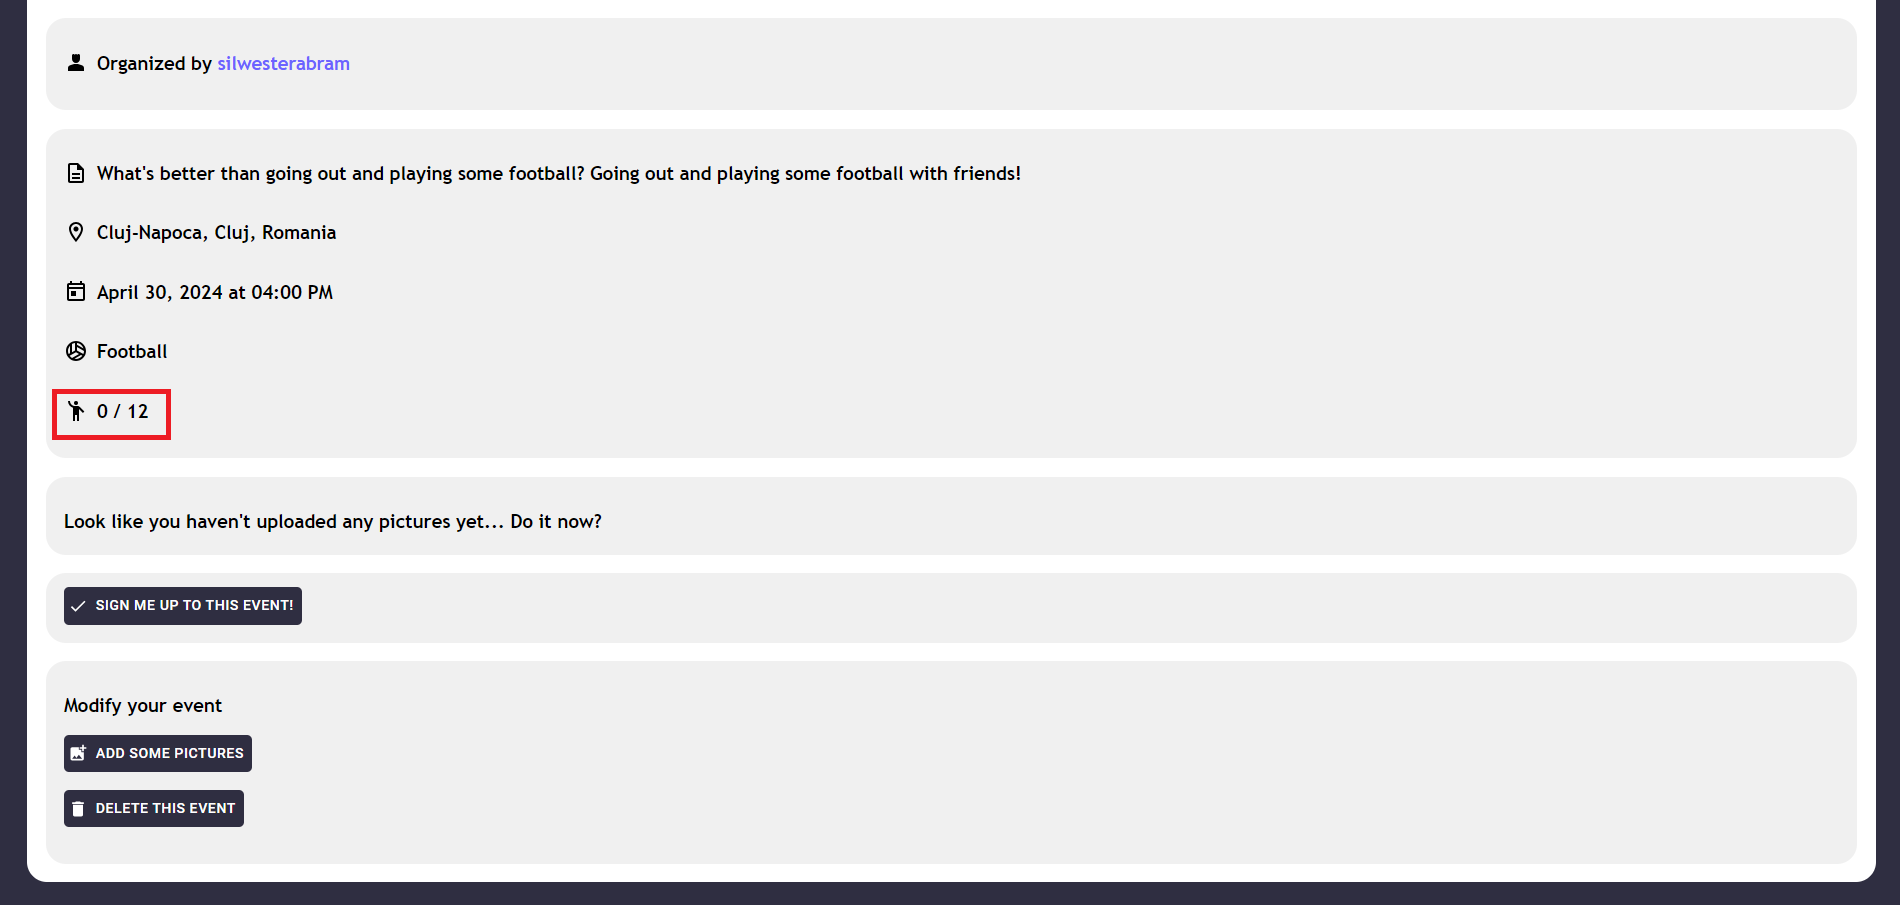
\includegraphics[width=0.5\textwidth]{images/resign_from_event_2.png}
	\caption{Egy eseményről való leiratkozás}
	\label{fig:resign_from_event}
\end{figure}

Szervezőként adhatunk hozzá képeket is az általunk szervezett eseményekhez. Ezt az ``Add some pictures'' gombra való kattintással tehetjük meg.
Ez felhoz egy ablakot, majd itt a képek kiválasztása után az oldal frissül és láthatóak lesznek az általunk kiválasztott képek. Ez a folyamat
látható a \ref{fig:add_pictures_event}-es ábrán.

\begin{figure}[ht]
	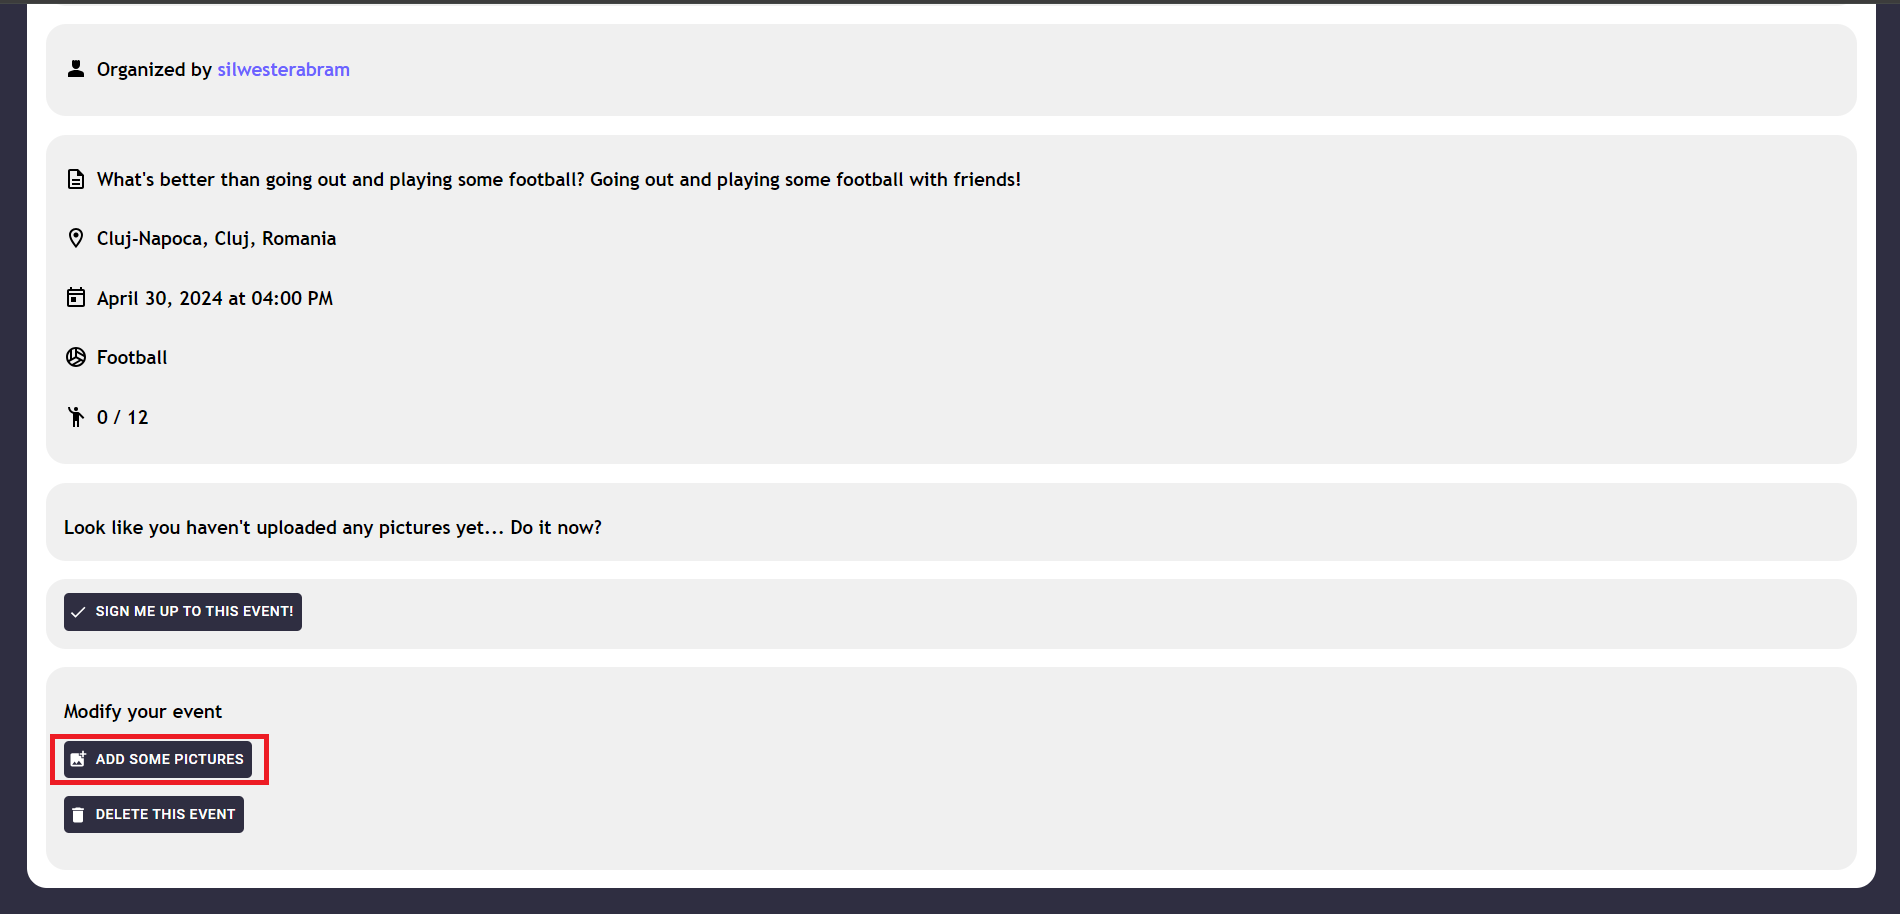
\includegraphics[width=0.5\textwidth]{images/add_pictures_event.png}
	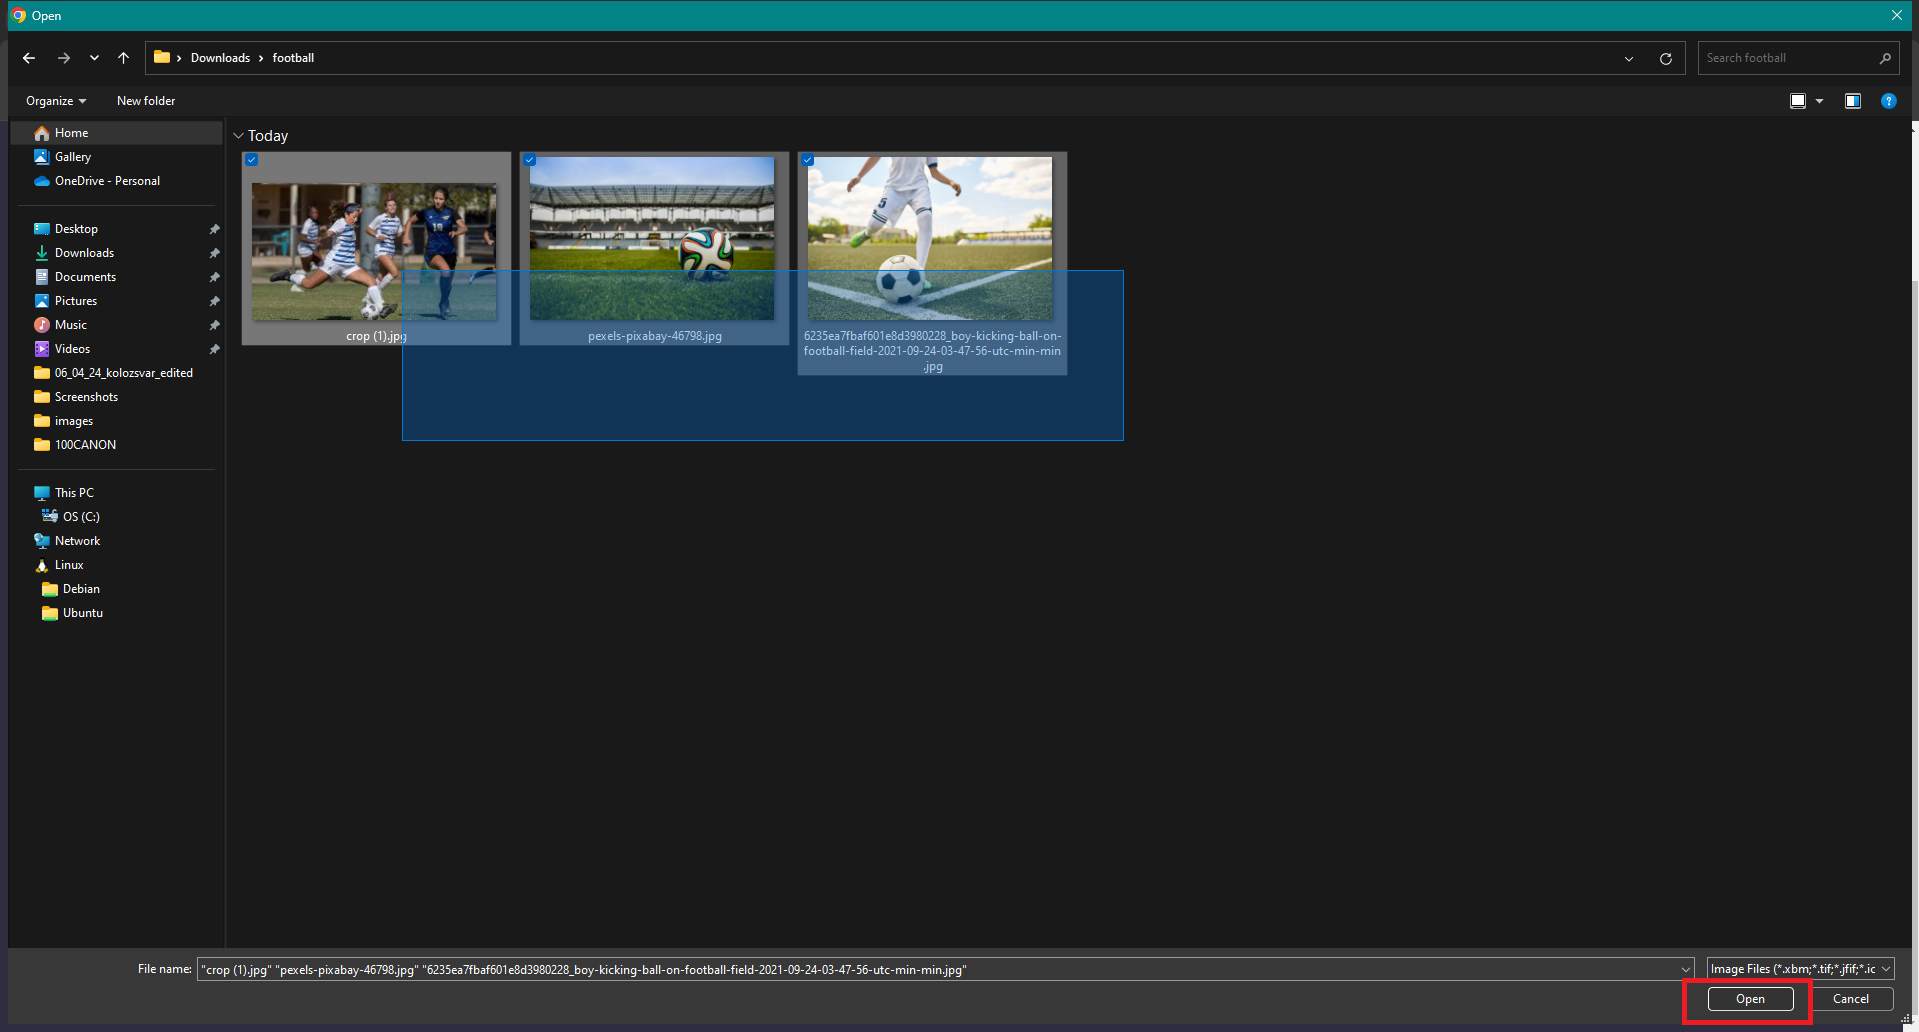
\includegraphics[width=0.5\textwidth]{images/add_pictures_event_2.png}
	\begin{center}
		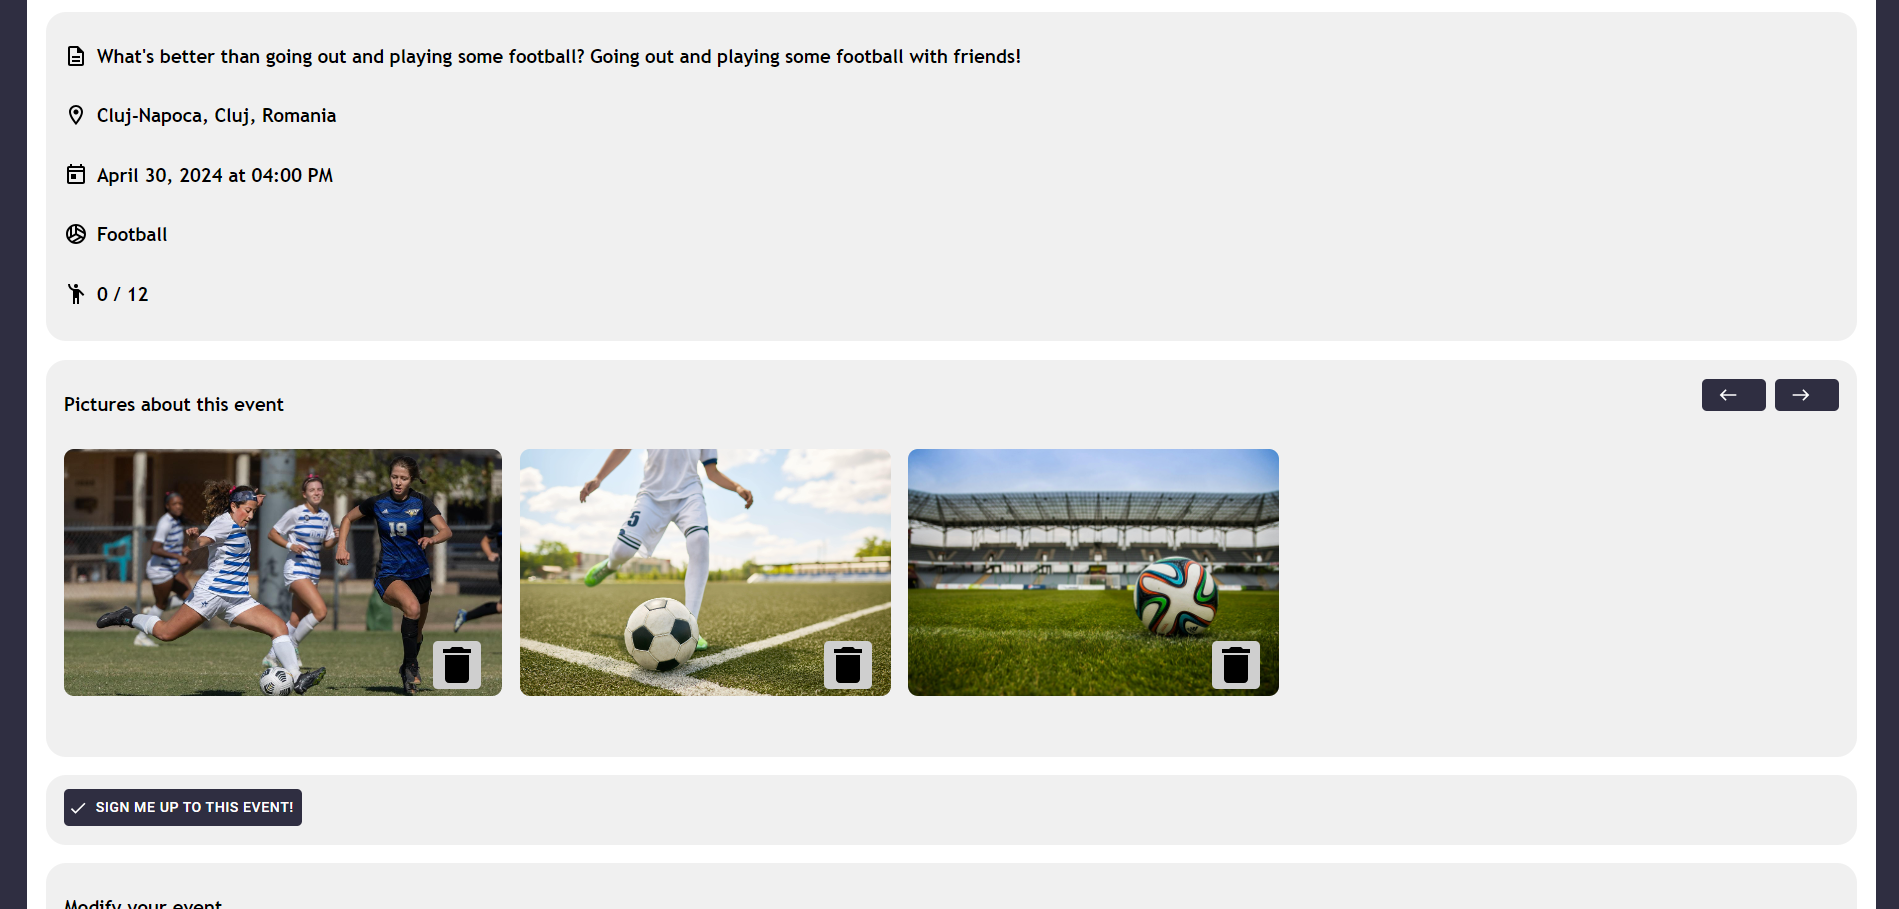
\includegraphics[width=0.7\textwidth]{images/add_pictures_event_3.png}
	\end{center}
	\caption{Képek hozzáadása az eseményhez}
	\label{fig:add_pictures_event}
\end{figure}

Egy esemény szervezője törölhet is képeket az eseményről. Ezt a kép jobb alsó sarkában megjelenő törlés ikonra kattintással teheti meg. Ilyenkor az oldal 
tartalma automatikusan frissül, s a törölni kívánt kép eltűnik az esemény oldaláról. Ez megfigyelhető a \ref{fig:delete_image_event}-as ábrán.

\begin{figure}[h]
	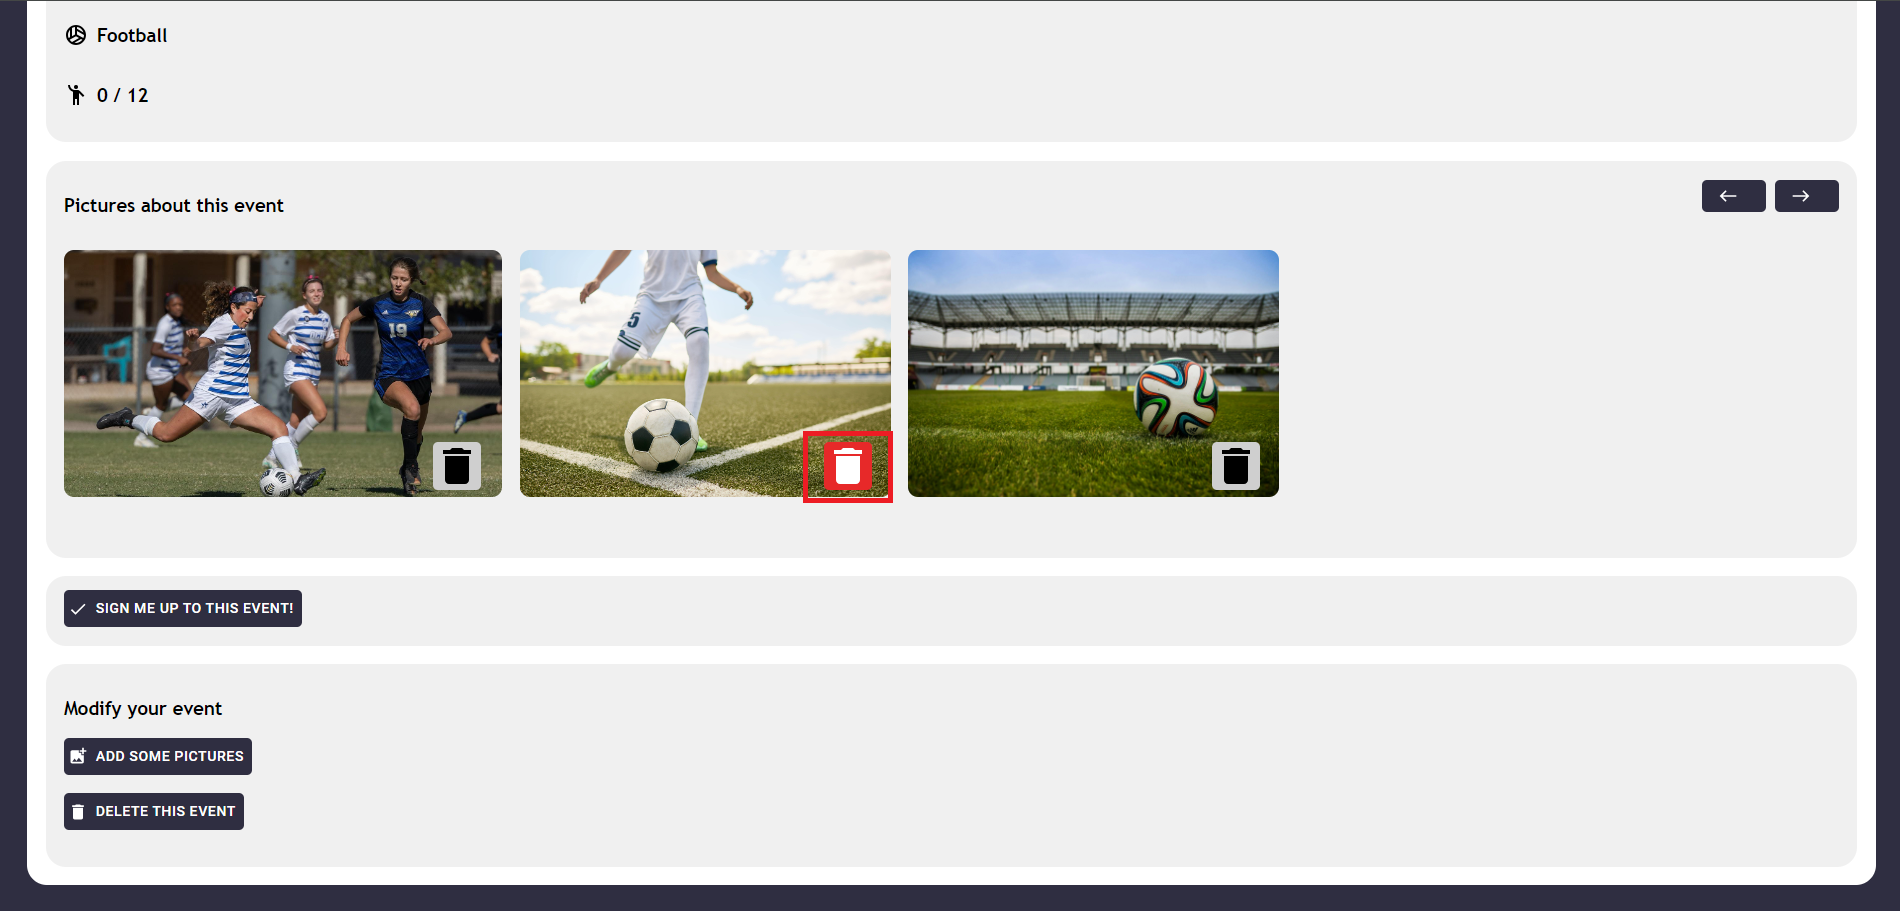
\includegraphics[width=0.5\textwidth]{images/delete_image_event_1.png}
	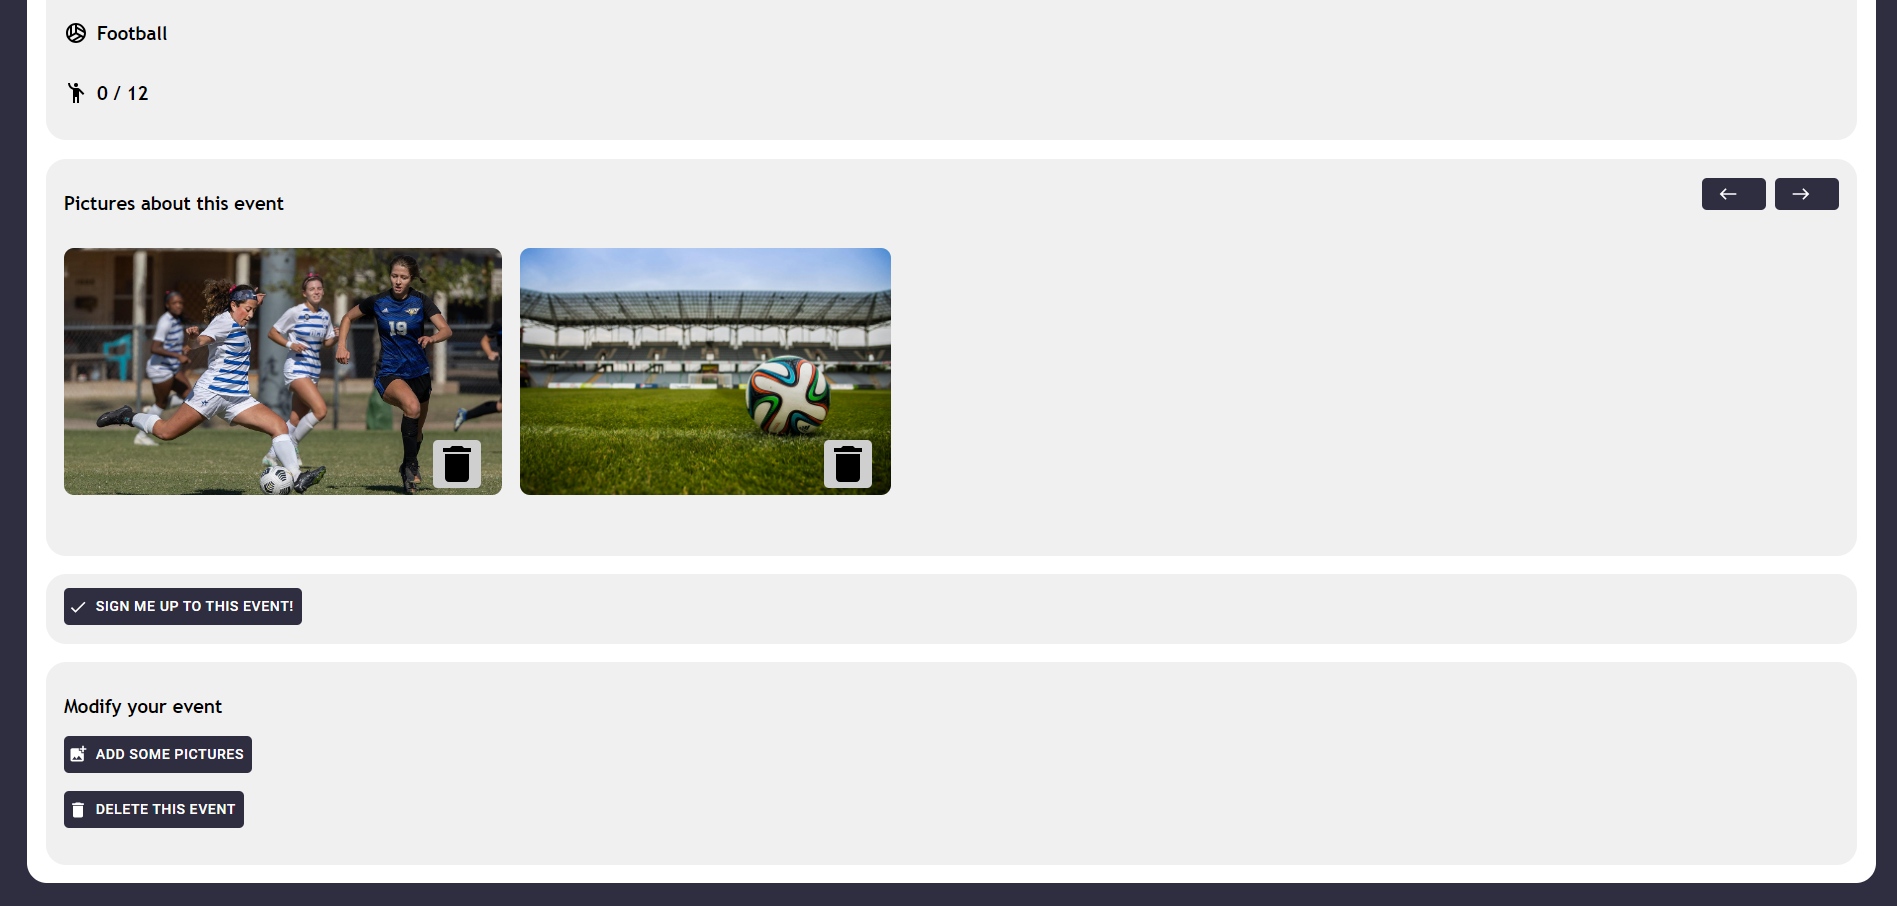
\includegraphics[width=0.5\textwidth]{images/delete_image_event_2.png}
	\caption{Kép törlése az eseményről}
	\label{fig:delete_image_event}
\end{figure}

Végső soron a szervező törölheti is az általa szervezett eseményt. Ezt a ``Delete this event'' gombra való kattintással teheti meg, ahogyan a \ref{fig:delete_event_details}-es ábrán is látható.
Ilyenkor egy megerősítendő ablak jelenik meg, amiben ha a ``Yes, delete this event!'' gombra kattintunk, az esemény véglegesen törlése kerül.
Ezután az oldal átirányít bennünket a böngésző felületre, ahol már nem fogjuk látni az általunk törölt eseményt.

\begin{figure}[ht]
	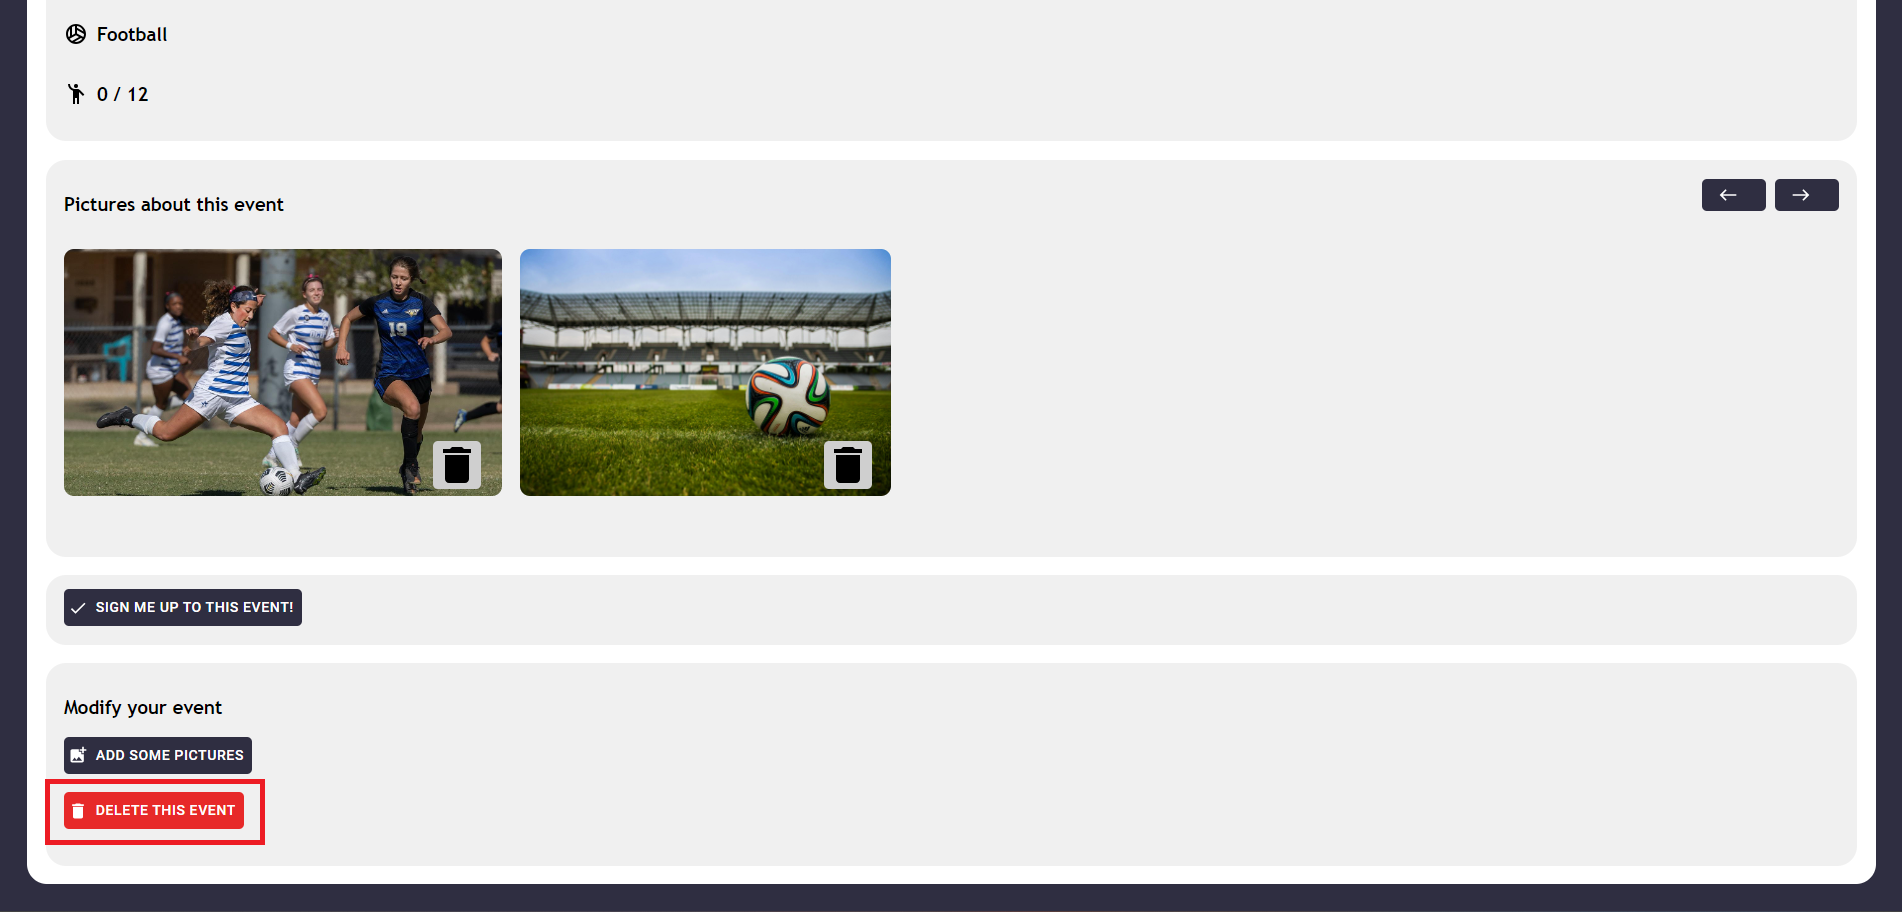
\includegraphics[width=0.5\textwidth]{images/delete_this_event_1.png}
	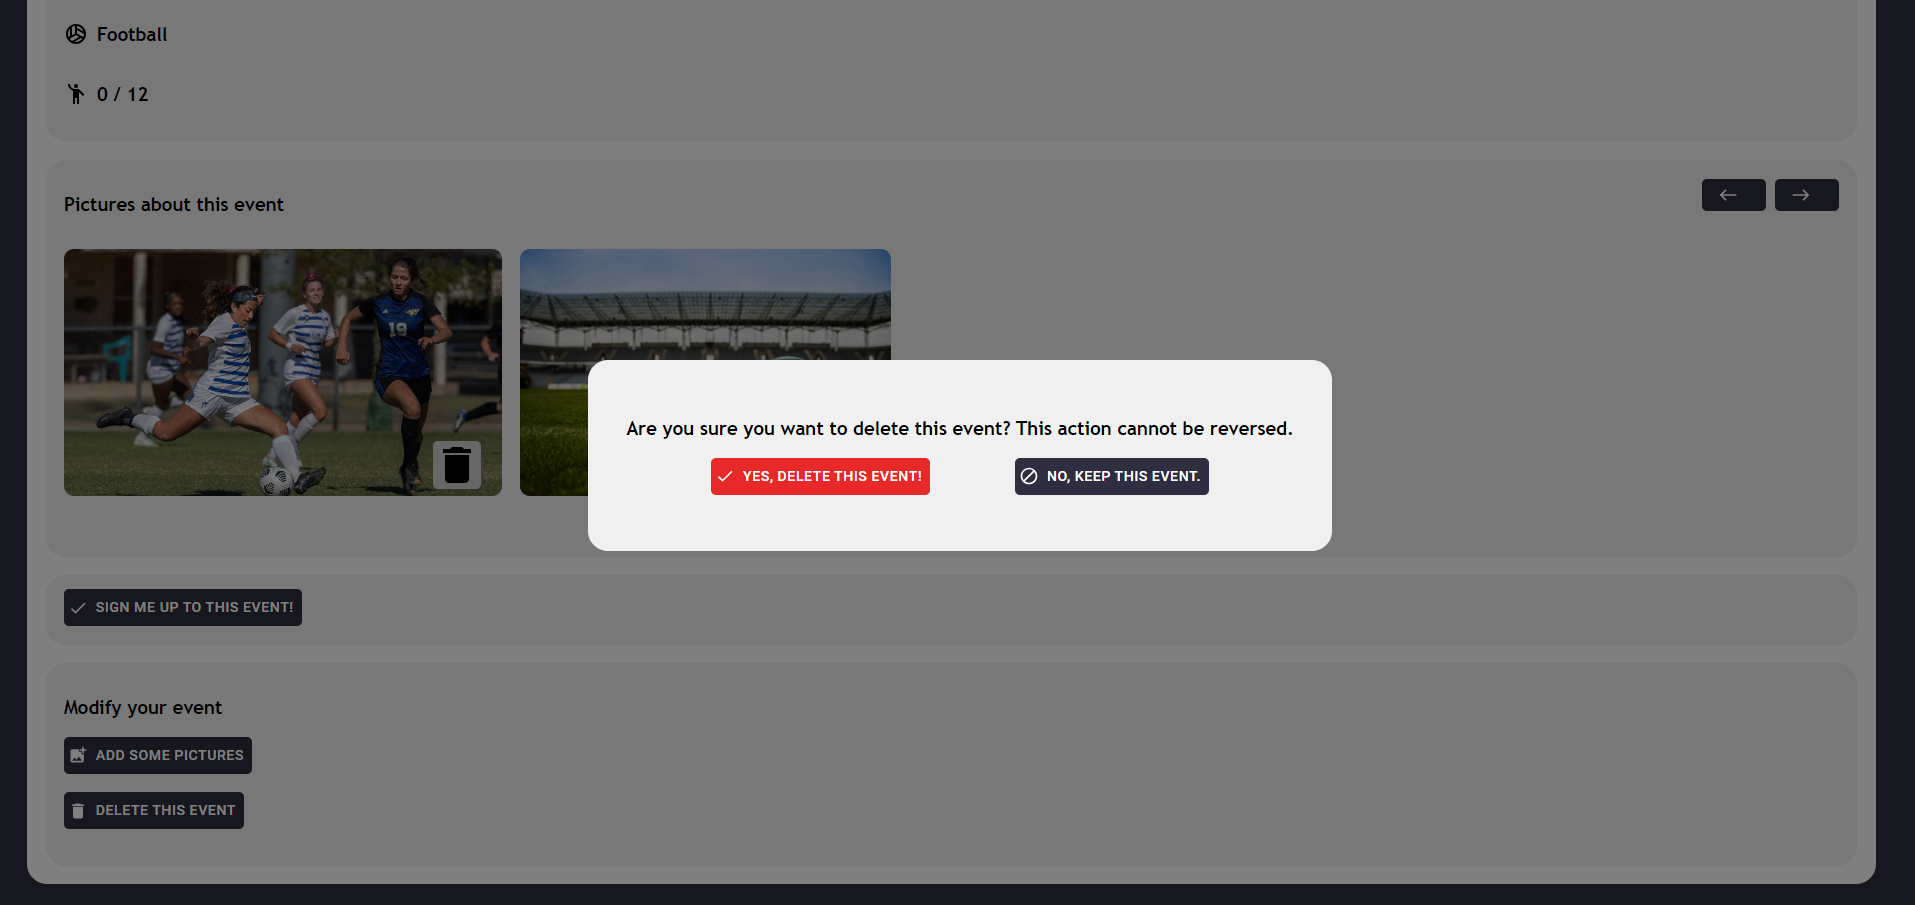
\includegraphics[width=0.5\textwidth]{images/delete_this_event_2.png}
	\caption{Esemény törlése}
	\label{fig:delete_event_details}
\end{figure}

\subsection{Sportesemények szűrése}

A sportesemények böngészése során a felhasználónak lehetősége van különböző szűrők használatára.
A szűrők segítségével meg lehet határozni egy időintervallumot, amely alatt az eseményeket meg szeretnénk tekinteni, illetve kiválasztható egy
specifikus sport is, amely alapján lehetősége van a felhasználóknak szűrni az eseményeket.

A szűrők használatához előszőr kattintsunk a ``Looking for something specific?'' fülre:

\begin{figure}[h]
	\centering
	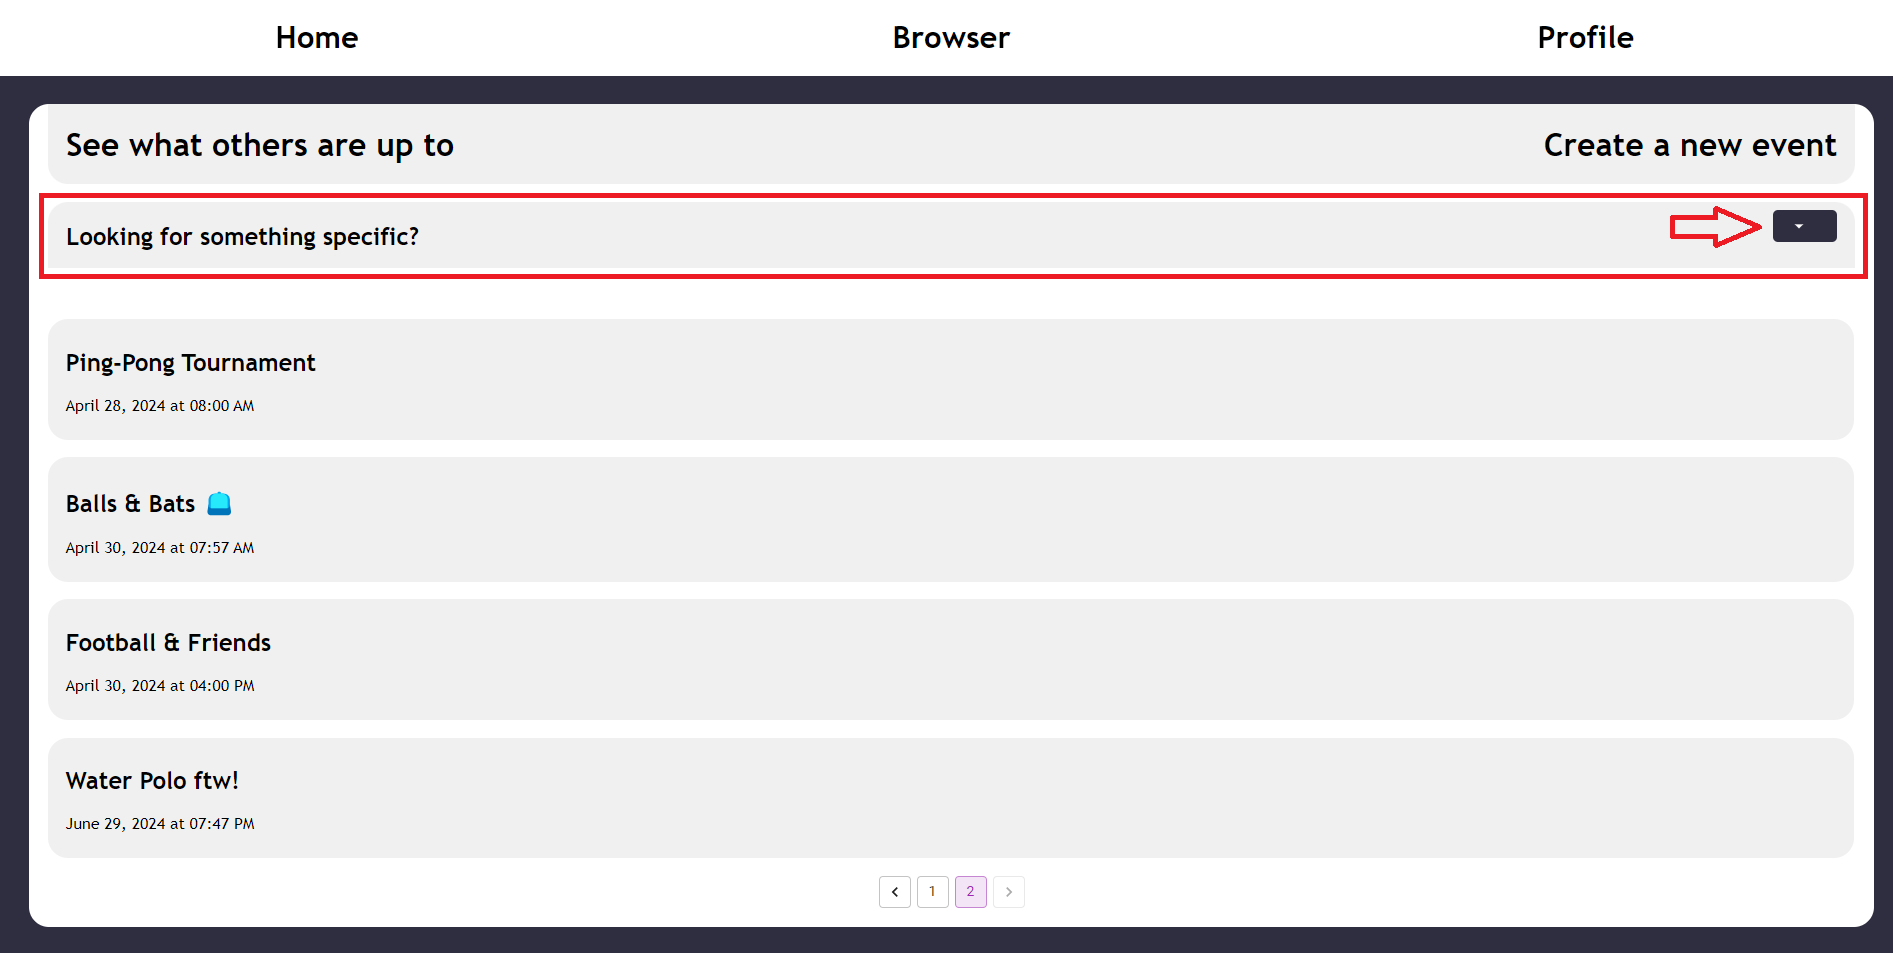
\includegraphics[width=0.5\textwidth]{images/filtering_events_1.png}
	\caption{A szűrőket tartalmazó fül előhozása}
	\label{fig:filter_1}
\end{figure}

\newpage

\begin{figure}[ht]
	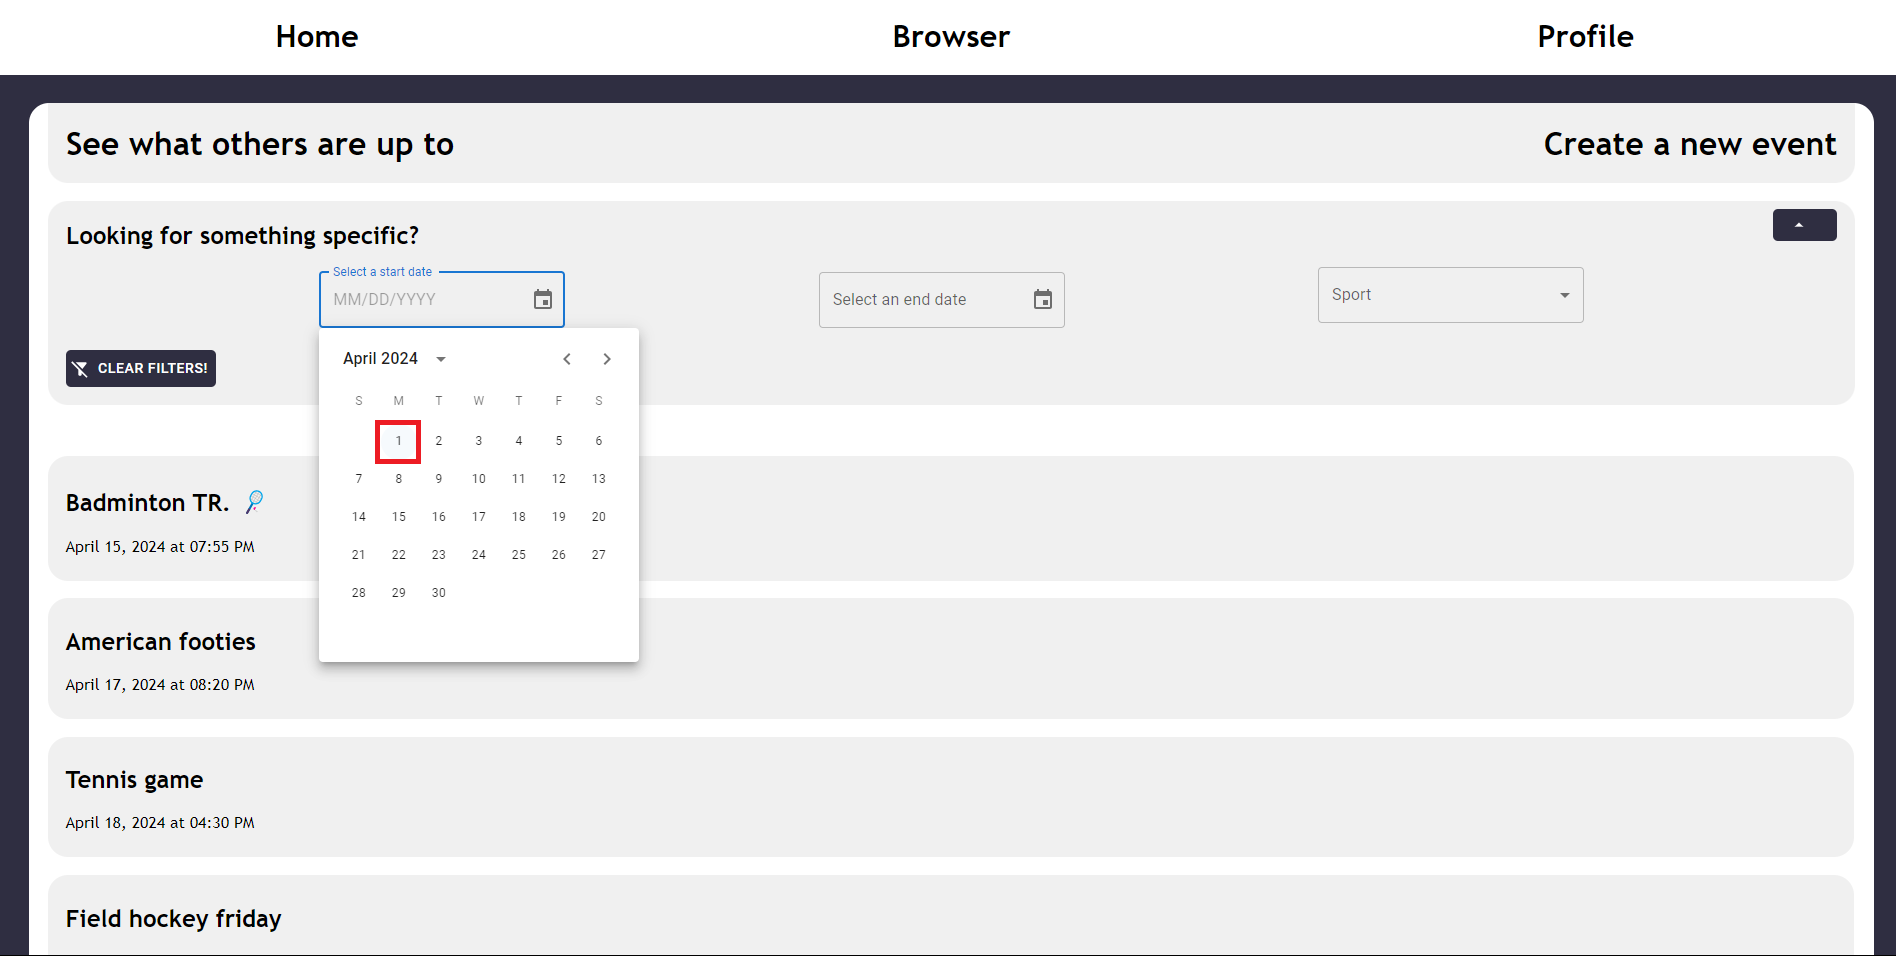
\includegraphics[width=0.5\textwidth]{images/filtering_events_2.png}
	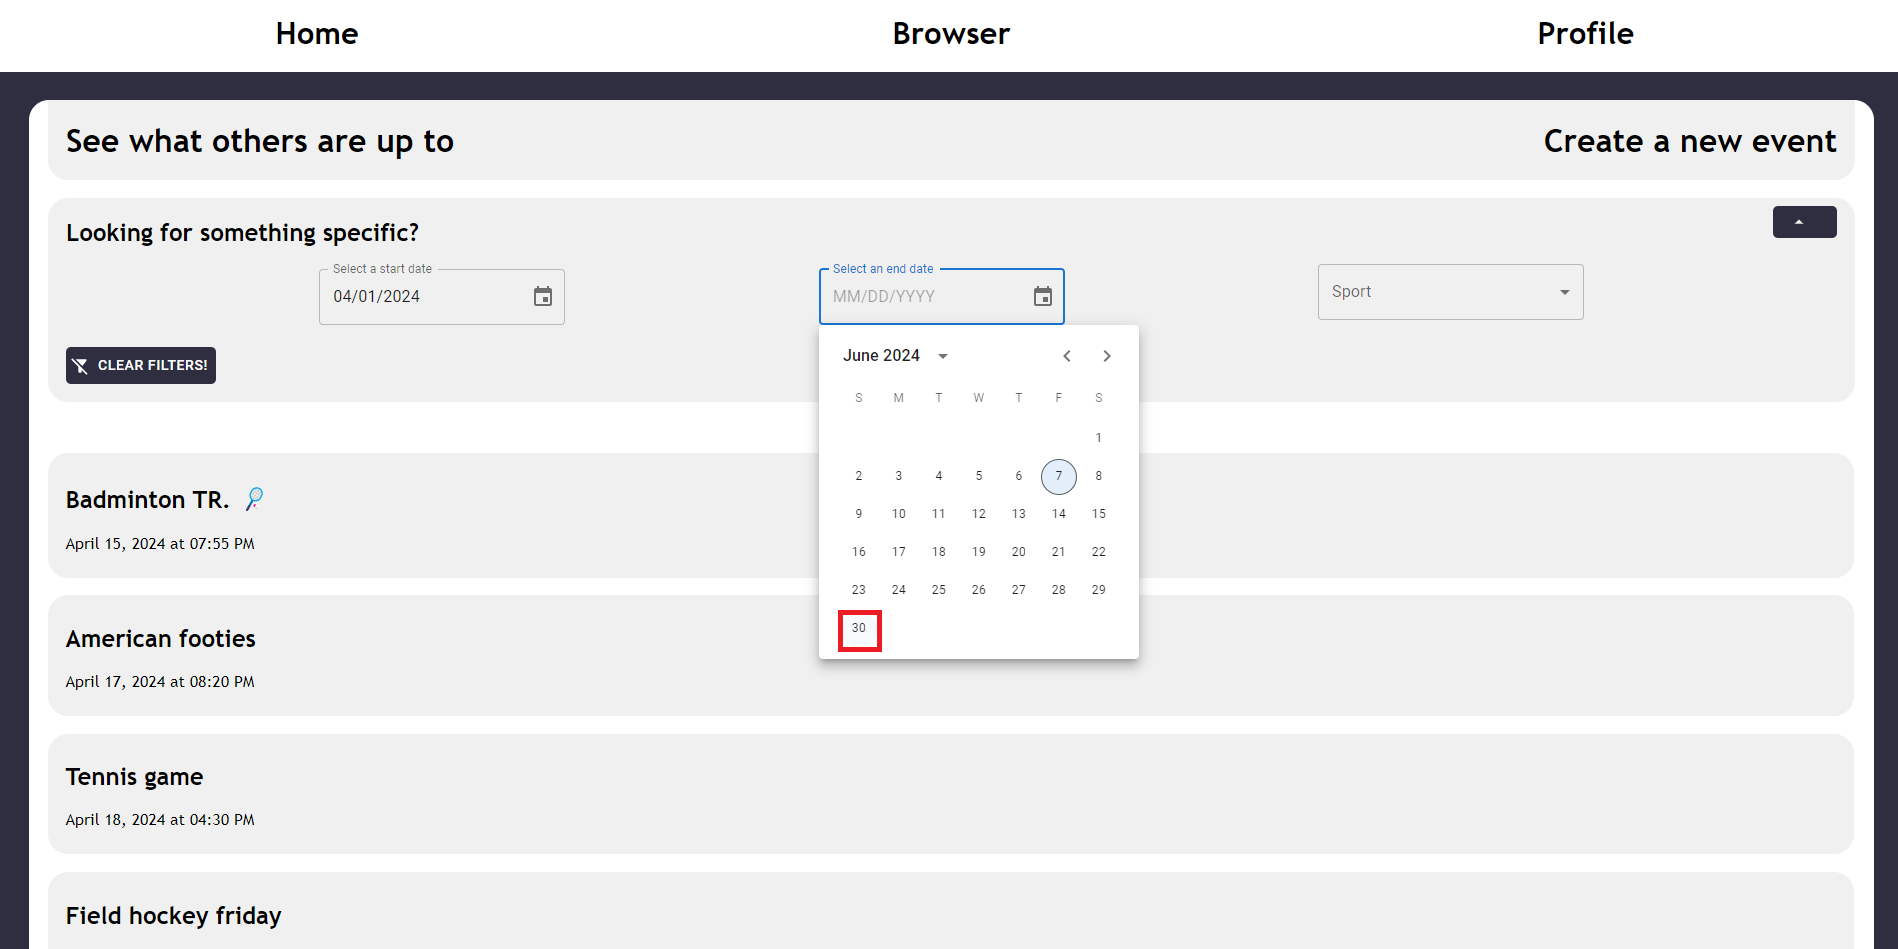
\includegraphics[width=0.5\textwidth]{images/filtering_events_3.png}
	\begin{center}
		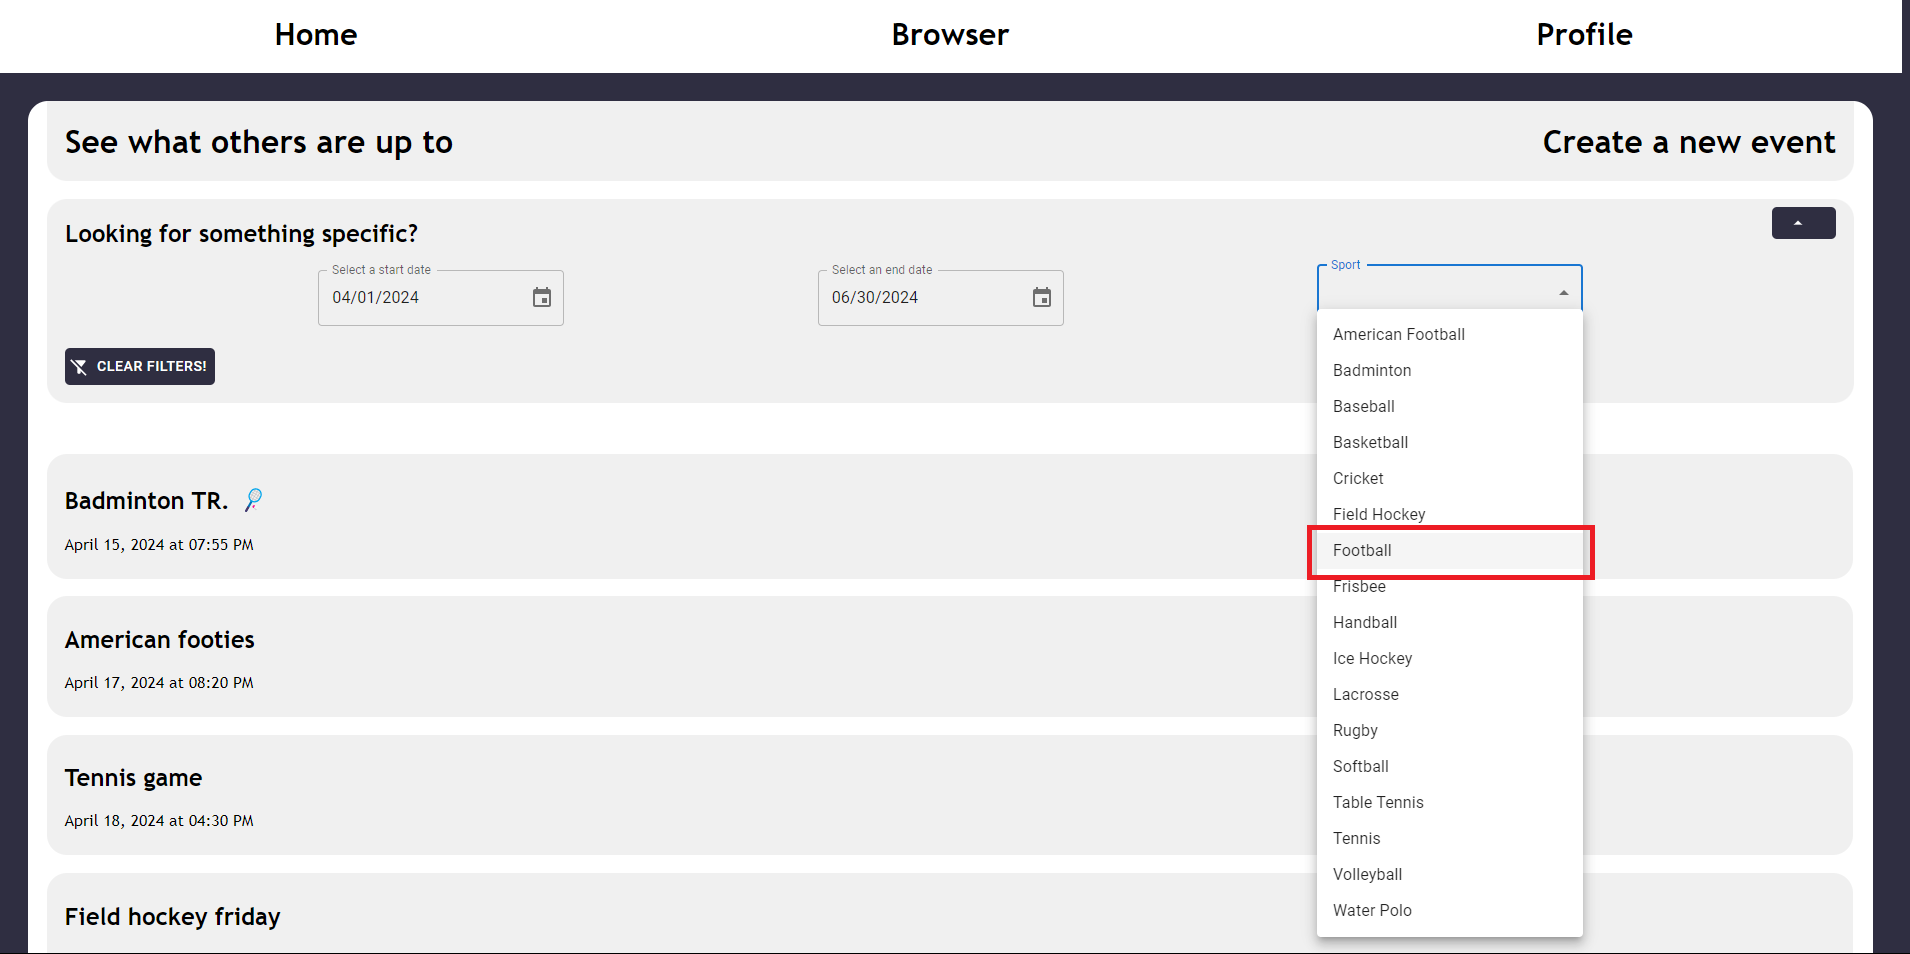
\includegraphics[width=0.5\textwidth]{images/filtering_events_4.png}
	\end{center}
	\caption{A szűrők beállítása}	
	\label{fig:applying_filters}
\end{figure}

Amint az látható a \ref{fig:applying_filters}-es ábrán, a szűrők beállítása után az oldal automatikusan frissül, és a beállított szűrőknek megfelelően
jeleníti meg az eseményeket. 

\begin{figure}
	\centering
	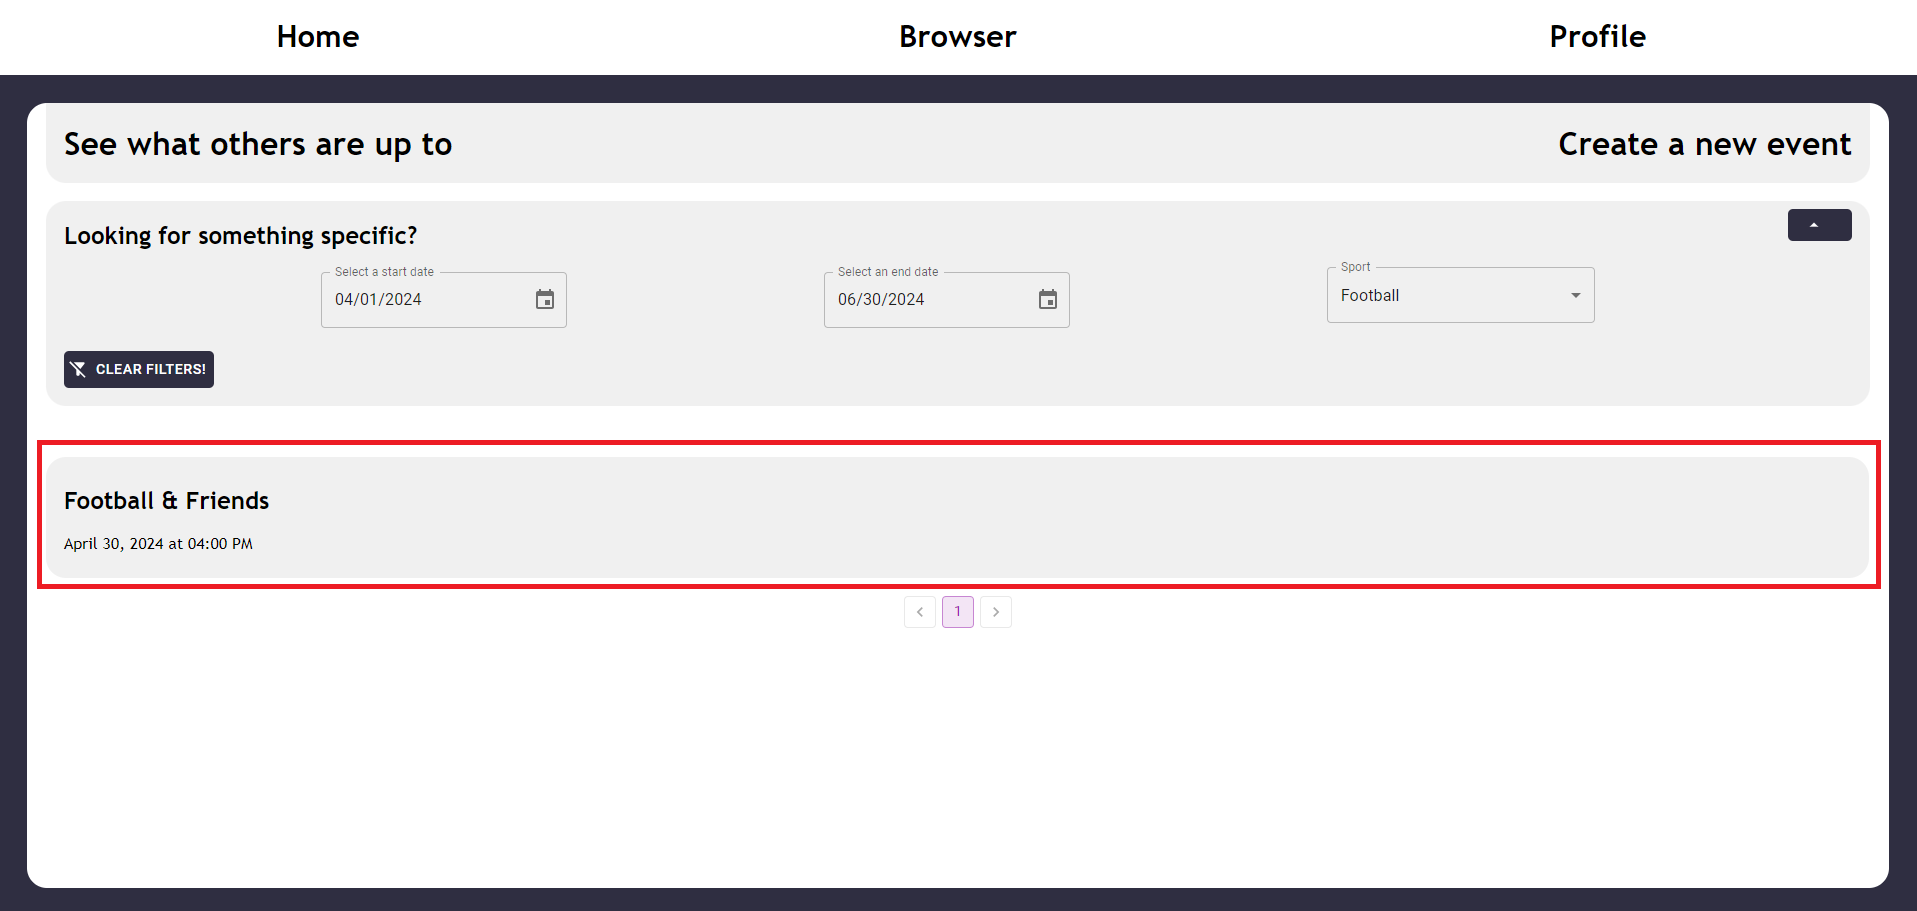
\includegraphics[width=0.7\textwidth]{images/filtering_events_5.png}
	\caption{A szűrt események}
	\label{fig:filtered_events}
\end{figure}

Ahogyan a \ref{fig:filtered_events}-es ábrán is látható, a szűrők alkalmazása egyetlen sporteseményt eredményezett.

\newpage
\section{Lapszámozás - Pagination}

Annak érdekében, hogy jó teljesítménnyel működhessen a webalkalmazás, szükséges az ú.n. \textit{Pagination}\cite{paginationdocs}, azaz az adatbázisból lekért sportesemények
szeletekre osztása. Ez azt jelenti, hogy nem fog minden felhasználó minden létező eseményt megkapni egy kérés során, hanem csak egy limitált számot,
melyek szekvenciális továbbá lekérhetőek.

Az alkalmazás automatikusan 5-ös szeletekre osztja a sporteseményeket, ezek között a lap alján van lehetősége a felhasználónak a navigálásra. Ez látható a \ref{fig:pagination}-os ábrán.

\begin{figure}[ht]
	\centering
	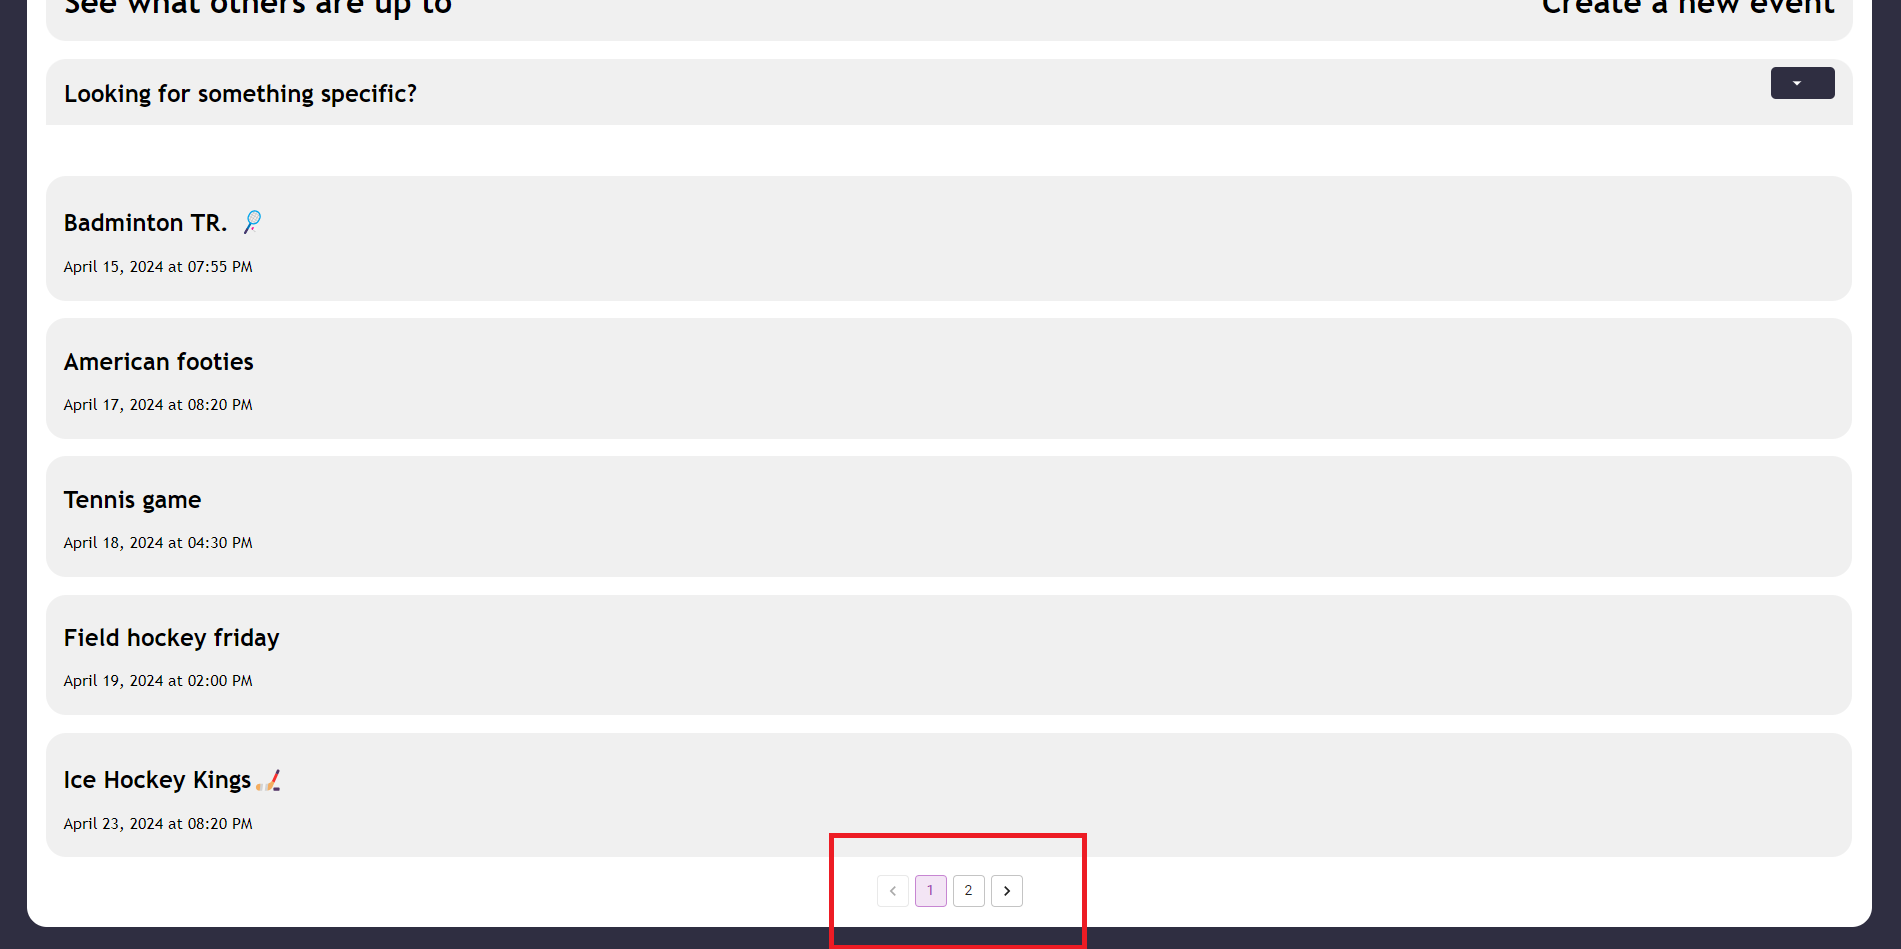
\includegraphics[width=0.7\textwidth]{images/pagination_1.png}
	\caption{A lapozás}
	\label{fig:pagination}
\end{figure}

Itt követehető az aktuális lap száma, illetve lehetőség van tovább haladásra a következő lapra, amennyiben ez létezik.